% GATE 3 WORKING DRAFT (not yet complete): 2026-11-05.
% Original 40-page paper + V16 are scientific coverage baselines.
% Core Gate 1/2 mathematical acceptance is scoped, not peer review.
% V16/V17 source and historical DOI must remain unchanged.
\IfFileExists{siamonline250211.cls}{%
 \documentclass[review,hidelinks,onefignum,onetabnum]{siamonline250211}%
 \def\isSIAM{1}%
}{%
 \documentclass[11pt]{article}%
 \def\isSIAM{0}%
}
% V17 uses the V16 SIAM manuscript interface. The article fallback is solely
% for offline preview when the repository's unchanged SIAM ZIP is unavailable.
\usepackage{microtype,xurl,needspace}
\usepackage{amsmath,amsfonts,amssymb,mathtools,bm}
\usepackage{graphicx,booktabs,enumitem,tabularx}
\usepackage[numbers,sort&compress]{natbib}
\ifnum\isSIAM=1
  \newsiamremark{assumption}{Assumption}
  \newsiamremark{remark}{Remark}
  \headers{When Can Markets Crash Without News?}{Siyuan Ye}
  \renewcommand{\footercopyright}{}
  \setlength{\headheight}{14pt}
\else
  \usepackage{amsthm}
  \usepackage[hidelinks]{hyperref}
  \usepackage[margin=1in]{geometry}
  \newtheorem{theorem}{Theorem}[section]
  \newtheorem{lemma}[theorem]{Lemma}
  \newtheorem{proposition}[theorem]{Proposition}
  \newtheorem{corollary}[theorem]{Corollary}
  \newtheorem{definition}[theorem]{Definition}
  \newtheorem{assumption}[theorem]{Assumption}
  \newtheorem{remark}[theorem]{Remark}
  \newcommand{\headers}[2]{}
  \newenvironment{keywords}{\noindent\textbf{Keywords.} }{\par}
  \newenvironment{MSCcodes}{\noindent\textbf{MSC codes.} }{\par}
\fi
\title{When Can Markets Crash Without News?\\Activity-Driven Recovery and Systemic Reachability}
\author{Siyuan Ye\thanks{Independent Researcher.}}
\hypersetup{pdftitle={When Can Markets Crash Without News? Activity-Driven Recovery and Systemic Reachability},pdfauthor={Siyuan Ye}}
\setlength{\emergencystretch}{2em}
\newcommand{\dd}{\,\mathrm{d}}
\newcommand{\Cris}{\mathcal{C}}
\newcommand{\one}{\mathbf{1}}
\newcommand{\pos}[1]{\left[#1\right]_+}
\newcommand{\TV}{\operatorname{TV}}
\begin{document}
\raggedbottom
\maketitle
\begin{abstract}
Matched-dollar transfers can produce systemic terminal price losses even when
fundamental benchmarks are fixed and every asset's cumulative executed-dollar
ledger closes at zero. We replace recovery in physical time by recovery driven
exclusively by gross executed-dollar activity. The resulting nonlinear control
system has no price motion without transactions. A nine-edge three-asset
protocol establishes local all-asset declines for arbitrary smooth positive
response functions, while scalar activity floors and execution-resource
inequalities restrict severe losses. Heterogeneous quadratic responses
can also produce a two-node systemic loss through a closed, sequential
dollar round trip, despite the homogeneous quadratic obstruction.
For homogeneous two-node power laws with $1<p\le3/2$,
a finite-size reversal produces systemic loss despite the
small-turnover barrier. For each fixed $K$, this finite-budget
region extends to a nonempty exponent interval above $3/2$
by continuity of the exact price-response flows.
One explicit $\mathsf C_1$ witness uses $p=5/4$, $K=1$
and only eight units of paired turnover. In the constant-impact model, a continuous-direction argument gives
an analytic existence construction for all ten prices to end at half
their benchmarks. For every fixed power-law exponent $0\le p<1$,
nine prices can become arbitrarily small under one common finite
turnover and inventory envelope (with constants depending on $p$).
A separate cross-checked internally interval-verified, no-instantaneous-netting ten-asset
path makes five assets close at the lower limit of successive $\pm25\%$
rolling sessions. The path has finite gross share-execution rate and an
equal-weight geometric-index loss above $16\%$. These are deterministic
reachability results, not equilibrium crash predictions.
\end{abstract}
\begin{keywords}market crashes; trade activity; price impact; systemic drawdown; reachability; interval verification; execution constraints\end{keywords}
\begin{MSCcodes}91G15, 91G45, 93B03, 65G30\end{MSCcodes}

\section{Introduction}\label{sec:intro}
Crashes may accompany public news, forced selling, liquidity withdrawal or
information revealed by trades. Their respective theoretical mechanisms are
studied, among others, by \citet{GennotteLeland1990,Romer1993},
\citet{HuangWang2009,CespaFoucault2014}, and \citet{ContWagalath2013}.
The predatory-trading mechanism studied by
\citet{BrunnermeierPedersen2005} introduces strategic reactions
that are intentionally absent from our model. These explanations
are distinct from a deterministic existence proof: they posit
endogenous information or incentives that may induce particular
trades, whereas we test which price endpoints are mechanically
compatible with the execution and settlement constraints.
An independent mathematical question is whether a price decline is compatible
with a fully paired stream of trades whose \emph{cumulative dollar balance
in each asset} is zero. This is a reachability question, not an explanation
of any particular historical crash.

Resilient execution models typically assign time dynamics to the liquidity
state; see \citet{ObizhaevaWang2013,AlfonsiSchied2010}. We instead ask what
changes when price resilience is triggered only by gross dollar activity
associated with actual trades. Such activity can be strictly positive even
when a node's simultaneous net executed-dollar flow vanishes. It is therefore
essential to distinguish a permissive control class from a stricter class
in which each node can only buy or only sell at a given instant. Our model
is an explicitly parameterized price-response law, not a strategic equilibrium
or a no-manipulation result of the type considered by
\citet{Gatheral2010,HubermanStanzl2004}.
Large-trader and liquidity-adjusted pricing frameworks
\citep{BankBaum2004,CetinJarrowProtter2004} offer a related
motivation for state-dependent execution responses, without
identifying their equilibria or supply curves with the
activity-driven law defined here.

We provide a self-contained analytic reachability chain and one narrow
computer-assisted construction. The universal results are local triangular
reachability, scalar floors, an aggregate full-coverage barrier, and necessary
turnover and inventory bounds. The ten-asset results are: (I) all ten
terminal prices equal one half of the benchmark; (II) nine losses have no
finite severity ceiling while time, turnover and inventory are bounded by
one set of constants; and (III) the same five assets close at the lower limits
of two consecutive $\pm25\%$ sessions under the stricter no-instantaneous-
netting class. The first two are analytic existence constructions whose
parameters need not coincide with the old physical-time model's numerical
budgets. We also derive a heterogeneous weighted-log balance and a
closed-ledger two-node counterexample; unlike the earlier physical-time
weighted-flow estimate, neither relies on a recovery term when no trades occur. The third has a reproducible, internally outward-rounded certificate.
No earlier fixed-version manuscript or its numerical certificate is
represented as a certificate for the present dynamics.

\section{The activity-driven paired-dollar market}\label{sec:model}
Fix $N\ge2$, a fixed benchmark $F>0$, positive transaction prices $S_i$,
and a positive locally $C^2$ response $g$. The complete bidirectional graph
without self-edges has incidence matrix $B$: for an edge from seller $i$ to
buyer $j$, $B_{ie}=-1$ and $B_{je}=1$. A control is a vector of nonnegative
edge-flow measures $\dd z_e$. The \emph{executed-dollar ledger} and \emph{gross
dollar activity} of asset $i$ are
\begin{equation}\label{eq:model}
 \dd X_i=\sum_e B_{ie}\dd z_e,\qquad
 \dd A_i=\sum_e|B_{ie}|\dd z_e,\qquad
 \boxed{\dd S_i=\frac{g(S_i)}{S_i}\dd X_i-\kappa(S_i-F)\dd A_i},\quad\kappa>0.
\end{equation}
The sums $\sum_i\dd X_i=0$, $\sum_i\dd A_i=2\sum_e\dd z_e$, and the
nodewise inequality $|\dd X_i|\le\dd A_i$ follow from incidence accounting.
A direct edge transfer of dollar mass $z>0$ is integrated in its own amount
parameter $a\in[0,z]$, including \emph{both} terms in \eqref{eq:model},
with $\dd\theta_i=\dd X_i/S_i$ for share positions. Finite sequences of such
flows and absolutely continuous rates are admissible while all intermediate
prices are positive. This flow-completed convention preserves the usual
chain rule; an old rule in which recovery freezes during a trade is \emph{not}
used here. Graph-completed impulsive-control systems provide a related
mathematical framework \citep{BressanRampazzo1988}, but the present
ordered-edge prescription is an explicit modeling assumption, not
a general assertion of path-order independence. If $\dd z=0$,
prices do not move.

\begin{definition}[Controls and execution resources]\label{def:controls}
In $\mathsf C_0$ every nonnegative edge flow is allowed, including simultaneous
inflow and outflow at one vertex. In $\mathsf C_1\subset\mathsf C_0$, each
asset is a pure dollar buyer or a pure dollar seller almost everywhere on
active periods; equivalently $|\dot X_i|=\dot A_i$ when $\dot A_i>0$.
Switching direction over time is permitted in both classes.
All paths start at $S_i(0)=F$ and impose $X_i(T)=0$ for \emph{every} asset.
The paired turnover and cumulative sales in shares are
\begin{equation}\label{eq:resource}
 M=\sum_e\int_0^T\dd z_e=\frac12\sum_i A_i(T),\qquad
 H_i^-=\sum_{e:\,B_{ie}=-1}\int_0^T\frac{\dd z_e}{S_i};
\end{equation}
when control is absolutely continuous the gross share-execution rate is
$r_i^{\rm gross}=\dot A_i/S_i$. In $\mathsf C_0$, $H_i^-$ counts
\emph{actual gross share sales} even when simultaneous purchases cancel
net executed dollars; the net negative variation of $X_i$ would undercount
those sales. Starting inventory $H_i\ge H_i^-$ prevents short sales.
Dollar closure does not require share-flatness.
\end{definition}

For power responses let
\begin{equation}\label{eq:power}
 g_p(S)=\eta(S/F)^p,\quad D_F=F^2/\eta,\quad
 x_i=S_i/F,\quad u_i=X_i/D_F,\quad a_i=A_i/D_F,\quad K=\kappa D_F.
\end{equation}
The uniquely relevant normalized dynamics are
\begin{equation}\label{eq:normalized}
 \boxed{\dd x_i=x_i^{p-1}\dd u_i-K(x_i-1)\dd a_i},\qquad
 |\dd u_i|\le\dd a_i,\quad\sum_i\dd u_i=0.
\end{equation}
In the power-law sections, dollars, shares, and prices are explicitly
normalized by $F=\eta=1$ where indicated. The absence of a calendar-time resilience term makes the following
time-scale statement exact; it replaces, rather than inherits, the
old physical-time model's critical-horizon theorem.

\begin{proposition}[No intrinsic horizon threshold without gross-rate caps]
\label{prop:time-change}
Fix the response law, the trading graph, the model parameters,
and a strictly positive admissible path on $[0,T]$, $T>0$,
formed from absolutely continuous nonnegative paired edge-dollar
rates and, optionally, finitely many ordered flow-completed edge
events, with finite turnover and genuine share inventories.
For every $T'>0$
there is an admissible path on $[0,T']$ in the \emph{same} class
$\mathsf C_0$ or $\mathsf C_1$ with precisely the same terminal
prices, individual terminal dollar ledgers, paired turnover, and
gross seller-share quantities. In particular, a terminal market
loss reachable on some positive horizon is reachable on every
positive horizon, so there is no nonzero \emph{calendar-time}
critical horizon in the model without a gross-rate constraint.
The conclusion does not imply that a loss state is reachable at
all; structural price and budget barriers still apply.
\end{proposition}
\begin{proof}
For an arbitrary $T'>0$ put $\lambda=T/T'$ and, for
$t\in[0,T']$, define
\[
 \widetilde S_i(t)=S_i(\lambda t),\quad
 \widetilde X_i(t)=X_i(\lambda t),\quad
 \widetilde A_i(t)=A_i(\lambda t),\quad
 \dot{\widetilde z}_e(t)
       =\lambda\dot z_e(\lambda t)\ge0.
\]
The absolutely continuous chain rule and the fact that
\eqref{eq:model} has no free $\dd t$ term show that these
transformed paths satisfy the same activity-driven model.
Their prices remain positive and every edge retains its
original incidence signs and transaction ordering.
The nodewise buyer/seller exclusivity required by
$\mathsf C_1$ is invariant under this positive time change.
For each of finitely many ordered flow-completed edge events,
transport its calendar timestamp $\tau$ to $\tau/\lambda$
while retaining its executed dollar amount and its relative
ordering. The event ODE is parameterized by executed dollar amount,
not elapsed time; hence its completed positive-price map and
share increment are identical before and after time rescaling.
Changing variables in the cumulative executed-dollar,
turnover and genuine gross share-sale integrals proves
\[
 \widetilde X_i(T')=X_i(T),\qquad
 \widetilde M=M,\qquad
 \widetilde H_i^-=H_i^-,\qquad
 \widetilde S_i(T')=S_i(T).
\]
Thus terminal dollar closure and systemic losses are unchanged.
By contrast, the gross share rate transforms as
$\widetilde r_i^{\rm gross}(t)
 =\lambda r_i^{\rm gross}(\lambda t)$.
Consequently the argument does not preserve a fixed cap
$r_i^{\rm gross}\le v$ when $\lambda>1$.
\end{proof}

\begin{definition}[Terminal systemic crisis]\label{def:crisis}
Write $L_i(T)=\log(F/S_i(T))$, $\bar L=N^{-1}\sum_iL_i$ and
$k=\lceil\alpha N\rceil$. If $Q_\alpha$ is the $k$th largest $L_i$, define
\begin{equation}\label{eq:crisis}
 \Cris_\alpha(T)=\min\{\bar L(T),Q_\alpha(T)\}.
\end{equation}
The terminal event is $\Cris_\alpha(T)\ge\delta>0$; neither rolling
peak drawdowns nor first-passage times are identified with this criterion.
\end{definition}

\subsection{Exact transformed accounting}
Define for positive prices
\begin{equation}\label{eq:coords}
 \Phi(S)=\int_F^S\frac{v}{g(v)}\dd v,\quad
 \Psi(S)=\int_F^S\frac{\dd v}{g(v)},\quad
 E(S)=\int_F^S\frac{v-F}{g(v)}\dd v\ge0,\quad
 R(S)=\frac{S(S-F)}{g(S)}.
\end{equation}
\begin{proposition}[The activity balance and execution cost]\label{prop:account}
For each flow-completed path,
\begin{align}
 \dd\Phi(S_i)&=\dd X_i-\kappa R(S_i)\dd A_i,\label{eq:phi}\\
 \dd\left[\sum_i\Phi(S_i)\right]&=-\kappa\sum_iR(S_i)\dd A_i,\label{eq:potential}\\
 X_i(T)&=F\,[\theta_i(T)-\theta_i(0)]+E(S_i(T))
  +\kappa\int\frac{(S_i-F)^2}{g(S_i)}\dd A_i.\label{eq:cost}
\end{align}
In particular, exact dollar closure and equal share positions both at $0$
and $T$ force a stationary price path. If $X_i(T)=0$ and $S_i(T)<F$,
then $\int_{S_i>F}R(S_i)\dd A_i>0$.
\end{proposition}
\begin{proof}
Use $\Phi'(S)=S/g(S)$ in \eqref{eq:model} to get \eqref{eq:phi};
paired transfers cancel in \eqref{eq:potential}. For the last identity,
$\dd X_i=S_i\dd\theta_i$ and
$\dd X_i-F\dd\theta_i=(S_i-F)\dd X_i/S_i
=(S_i-F)\dd S_i/g(S_i)+\kappa(S_i-F)^2\dd A_i/g(S_i)$.
Integrate and apply the chain rule to $E$.
The last two nonnegative terms in \eqref{eq:cost} must both vanish under
simultaneous closures. For $S_i(T)<F$, \eqref{eq:phi} with $X_i(T)=0$
implies $-\Phi(S_i(T))=\kappa\int R(S_i)\dd A_i>0$;
$R$ is positive only above $F$.
\end{proof}

\section{Local all-asset reachability}\label{sec:local}
For $g_p$ set
\begin{equation}\label{eq:w}
 w_p(x)=\int_1^x s^{1-p}\dd s
 =\begin{cases}(x^{2-p}-1)/(2-p),&p\ne2,\\ \log x,&p=2,\end{cases}
 \qquad r_p(w_p(x))=x^{1-p}(x-1).
\end{equation}
Then $\dd w_i=\dd u_i-Kr_p(w_i)\dd a_i$ with
$r_p(0)=0$ and $r_p'(0)=1$. The same linearization works for a general
smooth positive $g$ after scaling executed dollars by $F^2/g(F)$.

\begin{theorem}[Triangular local reachability]\label{thm:triangle}
On the complete bidirectional graph, for every $N\ge3$, $\kappa>0$
and every positive $C^2$ response $g$ near $F$, a finite $\mathsf C_1$
sequence has strictly positive intermediate prices,
$X_i(T)=0$ for every $i$, and $S_i(T)<F$ for every $i$.
For a normalized power response its prices satisfy
$w_i(T)=-m_iKz^2+O_N(z^3)$ as $z\downarrow0$, with
$m_1=m_2=N-2$ and $m_j=1$ for $j\ge3$.
\end{theorem}
\begin{proof}
On a triple $(a,b,c)$ execute nine equal-mass oriented edges, in order:
\[
 a\to b,\ b\to c,\ c\to a,\ b\to c,\ c\to a,\ a\to b,\ c\to a,\ a\to b,\ b\to c.
\]
Each vertex receives and sends exactly $3z$. Its six signs in its own
activity clock are respectively
$(-,+,+,-,+,-)$, $(+,-,-,+,+,-)$, and $(+,-,+,-,-,+)$.
All three satisfy $\sum_j\sigma_j=0$ and $\sum_jj\sigma_j=-1$.
In the transformed coordinate $r(w)=w+O(w^2)$, hence variation of
constants gives
\begin{align*}
 w(6z)&=\sum_{j=1}^6\sigma_j
 \int_{(j-1)z}^{jz}e^{-K(6z-a)}\dd a+O(z^3)\\
 &=Kz^2\sum_{j=1}^6j\sigma_j+O(z^3)=-Kz^2+O(z^3).
\end{align*}
Repeat the same triple protocol on $(1,2,j)$ for $j=3,\ldots,N$.
The shared vertices start the later protocols only $O(z^2)$ away from
benchmark, so subsequent increments retain the displayed quadratic
term; $m_i$ counts participation. Each edge is a one-directional sale/purchase
at the instant of execution, hence it is in $\mathsf C_1$. For sufficiently
small $z$ the full path stays in a compact positive price neighborhood;
initial inventories covering its finite sales suffice.
\end{proof}

\begin{remark}
The distinction between $N\ge3$ and $N=2$ matters. If $N=2$ then both
assets have identical activity clocks. If $e(S)=Sg'(S)/g(S)\ge1$ on the path,
concavity of $\Phi$ gives $R(S)\le\Phi(S)$ and
$\dd H\ge-\kappa H\dd A$, where $H=\sum_i\Phi(S_i)$ and $A$ is the common
clock. Since $H(0)=0$, simultaneous losses of both assets are impossible.
If $e\ge2$, concavity of $q\mapsto\Phi(Fe^q)$ also excludes
$\Cris_\alpha>0$ by Jensen's inequality. Neither is a general
$N\ge3$ obstruction in this activity model.
\end{remark}


\section{The two-asset boundary and partial coverage}\label{sec:twoasset}
The distinction between two and three assets does not arise from the number
of possible signs in a dollar ledger: it arises from the fact that both assets
of a two-node market must share the \emph{same gross activity clock}. In a
three-node market, one edge can change the activity of two nodes without
changing the third. The resulting heterogeneity permits the nine-edge
construction of Theorem~\ref{thm:triangle}.

\begin{proposition}[Two-node common-clock barriers]\label{prop:two-node-barriers}
Suppose $N=2$ and the response elasticity
$e(S)=Sg'(S)/g(S)\ge1$ on the positive-price state domain traversed
by an admissible dollar-closed path. Then both final prices cannot be
strictly less than $F$. If also $e(S)\ge2$, then
$\overline L(T)\le0$, and hence $\Cris_\alpha(T)\le0$ for every
$0<\alpha\le1$.
\end{proposition}
\begin{proof}
Every admissible edge increments both gross activity clocks equally,
including when opposite edges are simultaneously active in $\mathsf C_0$.
Let the common clock be $a$. Define $H=\Phi(S_1)+\Phi(S_2)$ and
$R(S)=S(S-F)/g(S)$. Because $\Phi''=(1-e)/g\le0$ and
$(R-\Phi)'=(S-F)\Phi''$, with $R(F)=\Phi(F)=0$,
one has $R(S)\le\Phi(S)$ for every $S$ in the state domain.
Thus $dH/da=-\kappa(R(S_1)+R(S_2))\ge-\kappa H$,
so $H\ge0$ by Gronwall from $H(0)=0$. Both prices below $F$
would imply $H<0$. If $e\ge2$, set $G(z)=\Phi(Fe^z)$.
Then $G'>0$ and $G''(z)=S^2[2-e(S)]/g(S)\le0$.
Concavity gives $G((\log(S_1/F)+\log(S_2/F))/2)\ge H/2\ge0$;
monotonicity of $G$ gives nonnegative mean log return.
\end{proof}

\begin{theorem}[A local two-node power-law classification]\label{thm:two-local}
Fix $N=2$, $K>0$ and a power-law exponent $p\ge0$.
For $0\le p\le1$, a sufficiently small dollar-closed two-edge
round trip has $\Cris_{1/2}(T)>0$; for $0\le p<1$,
its average terminal log loss is
\begin{equation}\label{eq:two-loss}
 \bar L=\frac{K(1-p)}{3}z^3+O(z^4)>0.
\end{equation}
For every fixed $1<p<2$ there exists $\varepsilon(p,K)>0$
such that \emph{no} terminally dollar-closed two-node path with total
paired turnover $A<\varepsilon$ can have positive mean log loss.
For $p\ge2$ no positive terminal systemic loss is possible, regardless
of the turnover budget. The result for $1<p<2$ is only a
\emph{small-turnover} exclusion, not an assertion of global
unreachability.
\end{theorem}
\begin{proof}
In node activity time $a$, write $w=(x^{\nu}-1)/\nu$,
$\nu=2-p$ (using $w=\log x$ if $p=2$) and
$r(w)=x^{\nu-1}(x-1)$. For a two-edge reversed transfer of
amount $z$ each, the two zero-order $w$ paths are $\pm a$
on $[0,z]$ and $\pm(2z-a)$ on $[z,2z]$. Since
\[
 r(w)=w-\tfrac12(p-1)w^2+O(w^3),
\]
the sum $H=w_1+w_2$ satisfies
$H(2z)=-(2/3)K(1-p)z^3+O(z^4)$ and each
terminal $w_i=O(z^2)$. Expanding $\log x_i=w_i+O(w_i^2)$
then proves \eqref{eq:two-loss}. One node has a strictly negative
terminal $w_i$ of order $z^2$, so the coverage condition also holds.
At $p=1$ the equation for $H$ is exactly $H'=-KH$,
therefore $x_1+x_2=2$ at the terminal time; the prices differ
on a nontrivial reverse pair and strict AM--GM gives $\bar L>0$.

For $1<p<2$, put $b(w)=w-r(w)$, so
$b(w)=(p-1)w^2/2+O(w^3)$. In a sufficiently small fixed
neighborhood of zero choose constants $c,L,C>0$ with
$b(w)\ge c w^2$, $|r(w)|\le L|w|$ and
$\log x(w)\ge w-Cw^2$. Under the shared gross clock $a\in[0,A]$,
$w_i'=\sigma_i-Kr(w_i)$, $|\sigma_i|\le1$,
$\sigma_1+\sigma_2=0$ and $\int_0^A\sigma_i\,da=0$.
Gronwall bounds $|w_i(a)|\le a\exp(KLa)$, so all admissible
controls stay in the chosen neighborhood for small enough $A$.
Let $J=\int_0^A(w_1^2+w_2^2)\,da$. Then
\[
 H(A)=K\int_0^A e^{-K(A-a)}\sum_i b(w_i(a))\,da
 \ge Kce^{-KA}J.
\]
Terminal ledger closure and Cauchy--Schwarz yield
$\sum_i w_i(A)^2\le K^2L^2AJ$. Consequently
\[
 \sum_i\log x_i(A)\ge
 K\{ce^{-KA}-CKL^2A\}J\ge0
\]
when $A$ is below a strictly positive threshold depending only
on $p,K$. Finally $p\ge2$ follows from Proposition~\ref{prop:two-node-barriers}.
\end{proof}

\begin{theorem}[Finite-budget two-node crises beyond the small-turnover barrier]
\label{thm:two-large-turnover}
Fix $N=2$, $F=\eta=1$, $K>0$ and $1<p<3/2$. There is
a strictly positive, terminally dollar-closed, sequential
$\mathsf C_1$ path of finite paired turnover, finite true
seller-side share inventory, and finite gross share-execution
rate for which $\Cris_{1/2}(T)>0$.
In particular, for $p=5/4$ and $K=1$ two reversed
four-dollar transfers at unit dollar rate on $[0,4]$
and $[4,8]$ give a fully explicit witness satisfying
\begin{equation}\label{eq:two-explicit-witness}
\begin{gathered}
 T=8,\quad M=8,\quad X_1(T)=X_2(T)=0,\\
 H_i^-<16,\quad \sup_{i,t}r_i^{\rm gross}(t)<4,\\
 S_1(T)S_2(T)<\frac{7555}{7716}<1,\qquad
 \Cris_{1/2}(T)>\frac12\log\frac{7716}{7555}>0.
\end{gathered}
\end{equation}
The lower bounds on initial shares and the upper rate bound
are genuine seller-side quantities, not net dollar variation.
\end{theorem}
\begin{proof}
Write $r=p-1\in(0,1/2)$ and use each node's
incident dollar amount as its activity clock. On an edge,
the buyer and seller prices respectively solve
\[
 \frac{\dd x}{\dd a}=f_+(x):=x^r-K(x-1),
 \qquad
 \frac{\dd x}{\dd a}=f_-(x):=-x^r-K(x-1).
\]
There is a unique attracting seller equilibrium
$x_-\in(0,1)$, since $f_-(0+)=K$, $f_-(1)=-1$,
and $f_-'(x)=-r x^{r-1}-K<0$.
There is also a unique attracting buyer equilibrium
$x_+>1$: the ratio $x^r/(x-1)$ is strictly
decreasing from $+\infty$ to zero on $(1,\infty)$.
The defining identity $K(x_+-1)=x_+^r$ yields
\[
 f_-(1/x_+)
 =x_+^{r-1}-x_+^{-r}<0
 \qquad (r<1/2).
\]
As $f_-$ is strictly decreasing, $x_-<1/x_+$,
so $x_-x_+<1$.

Transfer $z$ dollars from asset 2 to asset 1, followed
by $z$ from asset 1 to asset 2, in two nonoverlapping
active periods of dollar rate one. The exact individual
dollar ledgers close after the second period, and the
path belongs to $\mathsf C_1$. Starting at $x_i=1$,
the first-period prices remain between $x_-$ and $x_+$.
The reversed second-period seller flow converges
uniformly toward $x_-$ for initial states in
$[1,x_+]$, while the buyer flow converges uniformly
toward $x_+$ for initial states in $[x_-,1]$.
This follows by scalar comparison with the respective
flows starting at the extreme endpoints of those compact
intervals. Therefore, as $z\to\infty$,
\[
 (x_1(2z),x_2(2z))\longrightarrow(x_-,x_+),
 \qquad x_1(2z)x_2(2z)\longrightarrow x_-x_+<1.
\]
Some finite $z$ consequently has negative mean terminal
log return. For $N=2$ and $\alpha=1/2$, the maximum of
the two losses is at least their mean, so
$\Cris_{1/2}=\bar L=-\frac12\log(x_1x_2)>0$.
Throughout the construction $x_i\ge x_->0$; hence
$M=2z$, $H_i^-\le z/x_-$ and
$r_i^{\rm gross}\le1/x_-$ are all finite.

For the promised explicit witness take $p=5/4$, $K=1$
and $z=4$. The strict rational fourth-power comparisons
\[
 (3/4)^4>1/4,\quad (2/3)^4<1/3,\quad
 (3/2)^4>5/2
\]
imply $1/4<x_-<1/3$ and $1<x_+<5/2$.
The seller flow satisfies $f_-'(x)<-1$, so
during the second four-dollar period,
\[
 x_1(8)-x_-\le
 e^{-4}(x_1(4)-x_-)<\tfrac52 e^{-4}.
\]
The second-period buyer price remains below $x_+<5/2$.
Since the positive exponential series gives
$e^4>\sum_{k=0}^{5}4^k/k!=643/15$, it follows that
\[
 x_1(8)x_2(8)
 <\frac52\left(\frac13+\frac52\frac{15}{643}\right)
 =\frac{7555}{7716}<1.
\]
Both prices always exceed $x_->1/4$. Each asset
sells exactly four dollars once, so its actual sale of
shares is less than $4/(1/4)=16$; the unit incident
dollar rate gives $r_i^{\rm gross}<4$.
Every asserted inequality in \eqref{eq:two-explicit-witness}
is therefore exact and independent of ODE numerical
integration.
\end{proof}

\begin{proposition}[The critical two-node exponent $p=3/2$ is also reachable]
\label{prop:two-critical-p}
For $N=2$, $F=\eta=1$, any $K>0$ and $p=3/2$,
there is a finite-dollar, terminally dollar-closed
two-edge reversal in $\mathsf C_1$ with strictly positive
$\Cris_{1/2}(T)$, finite actual seller-side inventory,
and a finite gross share-execution rate.
\end{proposition}
\begin{proof}
Use the scalar buyer/seller flows $x'=f_\pm(x)$ from
Theorem~\ref{thm:two-large-turnover}, now with $r=p-1=1/2$.
Their stable positive equilibria satisfy $x_-x_+=1$,
because $f_-(1/x_+)=0$.
The positive magnitudes of the linearized relaxation
rates are
\[
 \gamma_-=-f_-'(x_-)
   =\frac K2\left(1+\frac1{x_-}\right),\qquad
 \gamma_+=-f_+'(x_+)
   =\frac K2\left(1+\frac1{x_+}\right).
\]
Since $x_-<1<x_+$, one has $\gamma_->\gamma_+>0$.

Write $\phi_\pm(a;y)$ for the scalar flow of
$x'=f_\pm(x)$ after executed-dollar activity $a$,
started from $x(0)=y$. After the first of two
opposite transfers of equal dollar amount $z$,
the first asset is in $[1,x_+]$ and the second
in $[x_-,1]$. Scalar order preservation gives
\[
 \begin{aligned}
 0<\Delta_-(z):=x_1(2z)-x_-
   &\le\phi_-(z;x_+)-x_-=:A(z),\\
 0<\Delta_+(z):=x_+-x_2(2z)
   &\ge x_+-\phi_+(z;1)=:B(z)>0.
 \end{aligned}
\]
For a scalar $C^1$ flow approaching a hyperbolic
stable equilibrium $x_*$ with $f'(x_*)=-\gamma$,
the logarithmic derivative of the positive distance
to equilibrium tends to $-\gamma$. Integrating
this logarithmic derivative and averaging over
the elapsed activity interval proves
\[
 \lim_{a\to\infty}
    \frac{1}{a}\log|x(a)-x_*|=-\gamma.
\]
Applying this result to $A(z)$ and $B(z)$
shows that $A(z)/B(z)\to0$, because
$\gamma_->\gamma_+$. Hence
$\Delta_-(z)/\Delta_+(z)\to0$, and for all
sufficiently large finite $z$,
\[
 x_1(2z)x_2(2z)-1
 =x_+\Delta_-(z)-x_-\Delta_+(z)
                     -\Delta_-(z)\Delta_+(z)<0.
\]
Thus $\Cris_{1/2}=-\tfrac12\log(x_1x_2)>0$.
The dollar ledgers close exactly, each asset's
true seller shares do not exceed $z/x_-$,
and unit dollar execution rate gives a finite
gross share rate at most $1/x_-$.
\end{proof}

\begin{corollary}[Reachability extends strictly beyond $p=3/2$]
\label{cor:nearcritical-beyond}
For every fixed $K>0$ there exists
$\varepsilon(K)\in(0,1/2)$ such that, for every exponent
$3/2\le p<3/2+\varepsilon(K)$, one and the same finite
two-edge dollar amount $z_K>0$ generates a terminally
dollar-closed $\mathsf C_1$ path with
$\Cris_{1/2}(2z_K)>0$.
The paths have strictly positive prices, finite
turnover $M=2z_K$, genuine seller-side share
inventories and finite gross share-execution rates
under unit dollar-amount-per-time scheduling.
No value of $\varepsilon(K)$ or sharp exponent
threshold is asserted here.
\end{corollary}
\begin{proof}
Fix $K>0$. Proposition~\ref{prop:two-critical-p}
provides a finite $z_K$ whose two consecutive
oppositely directed transfers, each of dollar amount
$z_K$, have terminal positive prices and strict
product $x_1(2z_K)x_2(2z_K)<1$ at $p=3/2$.
The entire reference trajectory is positive and
continuous on the compact amount interval
$[0,2z_K]$, and therefore has a positive minimum
price. On a compact positive neighborhood of this
reference path, the two scalar edge-flow vector
fields
\[
 f_\pm(x;p)=\pm x^{p-1}-K(x-1)
\]
are continuously differentiable in $(x,p)$.
Standard continuous dependence of ODE solutions
on parameters, applied successively to both
fixed-dollar stages, implies uniform convergence
of the trajectories and convergence of their
terminal-price products as $p\to3/2$.
The strict terminal product inequality persists
throughout some one-sided interval
$[3/2,3/2+\varepsilon(K))$.
After narrowing that interval if needed, every
price along the two events exceeds half the
positive minimum reference price. Thus true
seller-side share consumptions and gross
share-execution rates are finite, uniformly in
$p$ on the stated interval. Both edges have
the same fixed positive dollar mass and opposite
directions, so the individual executed-dollar
ledgers close exactly for all such $p$, and
$\mathsf C_1$ holds at every active time.
For two assets at $\alpha=1/2$, a terminal
price product below one gives positive
$\Cris_{1/2}$, as required.
\end{proof}

\paragraph{The remaining two-node global boundary.}
For $1<p\le3/2$, Theorems~\ref{thm:two-local},
\ref{thm:two-large-turnover} and
Proposition~\ref{prop:two-critical-p} establish a genuine
turnover-dependent reachability transition; by
Corollary~\ref{cor:nearcritical-beyond}, this positive
region extends slightly above $p=3/2$ for each fixed $K$: sufficiently
small dollar-closed round trips are obstructed, yet an
appropriate finite larger round trip succeeds. The
global reachability question for the remaining
$p\in[3/2+\varepsilon(K),2)$ is \emph{not}
classified by these results, and neither
the minimum successful turnover nor the full
$p,K,N$ and graph-topology phase diagram is claimed.

\section{Floors, aggregate barriers and execution resources}\label{sec:resources}
\begin{theorem}[Scalar activity-driven price floors]\label{thm:floor}
For the power response $g_p$, every individual normalized price is
bounded from below by the largest root $r\in(0,1)$ of
$K(1-r)=r^{p-1}$ whenever such a root exists. More precisely:
(i) if $p<1$, a strictly positive floor occurs for
\begin{equation}\label{eq:kc}
 K\ge K_c(p)=\frac{(2-p)^{2-p}}{(1-p)^{1-p}};
\end{equation}
(ii) for $p=1$ it occurs if $K>1$, and equals $1-1/K$;
(iii) for $p>1$ it occurs for every $K>0$.
For $p=0$, $K_c=4$ and the upper root is
$r=(1+\sqrt{1-4/K})/2$.
\end{theorem}
\begin{proof}
Using activity as clock and $|\dd u/\dd a|\le1$, the lowest possible
drift in $(0,1)$ is
$\dd x/\dd a\ge K(1-x)-x^{p-1}=:f_-(x)$.
A root of $f_-$ is a one-sided barrier by scalar comparison and local
ODE uniqueness. For $p<1$, minimize
$x^{p-1}/(1-x)$ on $(0,1)$ to get \eqref{eq:kc}, including the
noncrossable double root at equality. For $p=1$ solve the linear
root equation. For $p>1$, $f_-$ decreases strictly from $K$ at zero
to $-1$ at one and has a unique positive zero.
\end{proof}

\begin{theorem}[Necessary full-coverage bound]\label{thm:aggregate}
For any finite-variation flow-completed control in $\mathsf C_0$,
$p<2$ and $x_i(0)=1$,
\begin{equation}\label{eq:aggregate}
 \sum_{i=1}^N x_i(t)^{2-p}\ge1.
\end{equation}
In particular all $N$ prices cannot simultaneously be no larger than
$e^{-\delta}$ unless $\delta\le(\log N)/(2-p)$.
\end{theorem}
\begin{proof}
Put $\nu=2-p>0$ and $H=\sum_i w_p(x_i)$.
At every state where $H\le(1-N)/\nu$, we have
$\sum_i x_i^\nu\le1$, whence every $x_i\le1$ and
$\dd H=-K\sum_i x_i^{1-p}(x_i-1)\dd a_i\ge0$.
Initially $H=0>(1-N)/\nu$; continuity and the inward-pointing
inequality forbid crossing below $(1-N)/\nu$.
The event-flow convention permits the same argument during every edge
of a finite-variation path. Rearrangement gives \eqref{eq:aggregate}.
\end{proof}

\begin{theorem}[Necessary resources]\label{thm:lower}
Suppose at least $k$ assets end at $S_i(T)\le s=Fe^{-\delta}<F$.
Then for any $\mathsf C_0$ control,
\begin{equation}\label{eq:bounds}
 M\ge k[-\Phi(s)],\qquad
 \sum_iH_i^-\ge k[-\Psi(s)].
\end{equation}
If $X_i(T)=0$ and initial shares $H_i$ are available, then
$E(S_i(T))\le F H_i$. If $R(S)\le R_{\max}$ for all $S\in[F,U]$
and $S_i(t)\le U$ throughout, a terminally dollar-closed asset ending
below $s$ must have above-benchmark activity
\begin{equation}\label{eq:above}
 \int_{S_i>F}\dd A_i\ge\frac{-\Phi(s)}{\kappa R_{\max}}
 \quad (R_{\max}>0).
\end{equation}
\end{theorem}
\begin{proof}
On the last downward excursion from $F$ to $s$,
$\dd\Phi=\dd X-\kappa R\dd A\ge\dd X$ since $R<0$ below $F$.
Thus the negative-dollar variation of each target is at least
$-\Phi(s)$; summing sellers counts each paired dollar transfer once.
Similarly, a downward price excursion below $F$ satisfies
$\dd S\ge-g(S)(-\dd\theta)_+$ and therefore requires at least
$-\Psi(s)$ sold shares. Cost identity \eqref{eq:cost} and
$\Delta\theta_i\ge-H_i$ give the inventory inequality.
Finally, $-\Phi(S_i(T))=\kappa\int R\dd A$
under dollar closure and its positive part can only arise above $F$;
there $R\le R_{\max}$. If $S_i(T)\le s$, the stated bound follows.
\end{proof}

\begin{theorem}[A $K$-dependent turnover lower bound]\label{thm:kresource}
For $p=0$, define $D_F=F^2/\eta$. If $k$ dollar-closed assets
end at or below $s=Fe^{-\delta}$, then
\begin{equation}\label{eq:Kbound}
 M\ge kD_F\sqrt{\frac{1-e^{-2\delta}}{2K(2+K)}}.
\end{equation}
In particular this necessary lower bound diverges as $K^{-1/2}$
when $K\downarrow0$ at a fixed positive target severity.
\end{theorem}
\begin{proof}
Normalize $F=\eta=1$ and use the $i$th node's activity clock
$a\in[0,2b]$. Dollar closure makes its total buys and sells equal $b$,
so its signed ledger obeys $u(0)=u(2b)=0$ and
$u(a)\le\min(a,2b-a)$. For $w=(x^2-1)/2$ and $r=x(x-1)$,
$\dd w=\dd u-Kr\dd a$. Since $r\ge-1/4$ and
$r\le2[w]_+$ for every $x>0$,
\[
 [w(a)]_+\le\min(a,2b-a)+Ka/4,
 \qquad \int_0^{2b}r\dd a\le(2+K)b^2.
\]
At the terminal time, $-w(T)=K\int r\dd a\ge(1-s^2)/2$.
Hence $b\ge\sqrt{(1-s^2)/[2K(2+K)]}$.
The sum of all dollar purchases equals paired turnover $M$.
Restore the executed-dollar unit $D_F$.
\end{proof}

\begin{proposition}[All-node second-session obstruction]\label{prop:second}
If all assets stay at or below $F$ throughout a second trading session,
they cannot all close that session strictly below their respective
opening prices, regardless of execution-rate bounds.
\end{proposition}
\begin{proof}
The activity potential obeys \eqref{eq:potential}, and every
$R(S_i)\le0$ throughout the session, hence $H$ cannot decrease.
Strict decline of every price would strictly decrease
$H=\sum_i\Phi(S_i)$, a contradiction.
\end{proof}


\section{Bounded gross share rates and local speed constraints}
\label{sec:rates}
A rate bound changes the admissible set: specify the \emph{gross}
share rate, not the rate of the net executed-dollar ledger,
\begin{equation}\label{eq:grossrate}
 \frac{\dot A_i(t)}{S_i(t)}\le v
 \quad\text{for almost every }t\in[0,T],\qquad v<\infty.
\end{equation}
Writing $h(S)=g(S)/S$, the pairing condition
$\sum_i\dot X_i=0$ cancels the first-order aggregate price
response at the common benchmark. This cancellation is local and
does not imply a conserved scalar over the full path.
Whereas optimal-execution studies such as
\citet{AlmgrenChriss2001,Yang2019} investigate how to choose
trading rates under cost and speed constraints, our gross
share-rate restriction is a \emph{reachability} constraint:
it rules out certain terminal losses without identifying an
investor's optimal trading policy.

\begin{theorem}[Conditional quadratic small-rate barrier]\label{thm:ratequadratic}
Let $I=[F-d,F+d]\subset(0,\infty)$ be a compact interval on
which $g$ is positive and $C^2$. Define
\[
 C_I=\sup_{S\in I}\{g(S)+\kappa S|S-F|\},\quad
 U_I=\sup I,\quad L_I=\sup_{S\in I}|h'(S)|.
\]
If $v C_IT<d$, every trajectory satisfying \eqref{eq:grossrate}
remains in $I$ and
\begin{equation}\label{eq:ratebarrier}
 |\bar S(T)-F|\le\frac12 v^2T^2 C_IU_I(L_I+\kappa),
 \quad \Cris_\alpha(T)\le\bar L(T)\le B_I v^2T^2,
\end{equation}
where $B_I$ is the explicit constant obtained by combining the
first bound with the Taylor inequality
$-\log(1+y)\le-y+y^2/[2(1-b)^2]$ for
$|y|\le b=v C_IT/F<1$. Thus a uniformly bounded-rate market
cannot produce a fixed positive terminal crisis severity on an
arbitrarily short, sufficiently regular horizon.
\end{theorem}
\begin{proof}
The inequalities $|\dot X_i|\le\dot A_i\le vS_i$ imply
$|\dot S_i|\le v C_I$ as long as $S_i\in I$. A first-exit
argument establishes invariance of $I$ under $vC_IT<d$.
Let $y_i=S_i-F$. Summing the price equations and subtracting
the common coefficient $h(F)$ from their trade terms gives
\[
 \dot{\bar S}=
 \frac1N\sum_i [h(S_i)-h(F)]\dot X_i
 -\frac\kappa N\sum_i(S_i-F)\dot A_i.
\]
Use $|y_i(t)|\le v C_I t$,
$|h(S_i)-h(F)|\le L_I |y_i|$ and
$\dot A_i\le v U_I$ and integrate $t$ from $0$ to $T$.
The logarithmic estimate and $\Cris_\alpha\le\bar L$
complete the proof. The same conclusion holds for either $\mathsf C_0$
or $\mathsf C_1$ control, since gross activity was retained throughout.
A rate-independent explicit constant under a fixed margin is given in
Proposition~\ref{prop:rate-explicit}, and a matching local quadratic
construction is supplied by Proposition~\ref{prop:rate-local-match}.
\end{proof}

\begin{proposition}[Pure-sale speed test]\label{prop:pure-sale}
Suppose the price falls from $s_0$ to $s_1<s_0$ during a
period of length $\tau$, and the gross share rate is bounded by $v$.
On a price interval where
$G_-(S)=g(S)+\kappa S(S-F)>0$,
a necessary condition is
\begin{equation}\label{eq:puresell}
 v\tau\ge\int_{s_1}^{s_0}\frac{dS}{G_-(S)}.
\end{equation}
In the normalized $p=0,K=2$ model,
$G_-(x)=2(x-\tfrac12)^2+\tfrac12$, so the integral equals
$\arctan(2s_0-1)-\arctan(2s_1-1)$.
\end{proposition}
\begin{proof}
A sale is the maximal instantaneous negative net-dollar flow,
$\dot X_i\ge-\dot A_i$. Thus
$-\dot S_i\le[g(S_i)/S_i+\kappa(S_i-F)]\dot A_i
\le vG_-(S_i)$ when $G_->0$. Integrate a decreasing
segment. The result is a \emph{necessary} scalar constraint; it does
not construct paired-dollar counterparties or close their ledgers.
\end{proof}

\paragraph{A bounded-rate local construction.}
Spread the nine-edge triangle of Theorem~\ref{thm:triangle}
over a fixed positive interval, assigning each edge its required
dollar amount at a sufficiently small positive rate. The price path
remains in a compact neighborhood of $F$, and each gross share
rate is of order $z/T$ while its terminal losses are of order
$z^2$. Thus the quadratic exponent in \eqref{eq:ratebarrier}
is locally attainable for $N\ge3$, though neither the constant nor
any severe-loss optimal execution is inferred from this local scaling.

\section{Rolling price limits, breadth, and market cuts}\label{sec:bands}
Suppose consecutive sessions are indexed by $d=1,\dots,D$.
Within each session, a price may not move beyond a fraction
$\ell\in(0,1)$ of its preceding close. Specifically, if
$s_{i,d-1}$ is the previous close, the entire session must satisfy
$(1-\ell)s_{i,d-1}\le S_i(t)\le(1+\ell)s_{i,d-1}$.
The next session's band is reset to the new close; the fundamental
benchmark $F$ is \emph{not} reset.
This repeatedly resetting percentage band is a stylized
mathematical constraint, not a claim about the detailed
tick-based daily limits of any specific exchange. Real
market schedules, including the domestic-equity rules
documented by Japan Exchange Group \citep{JPX2026},
may be price-level dependent; the $\pm25\%$ scenarios
below are therefore hypothetical stress constraints.

\begin{proposition}[Exact cross-sectional compensation criterion]
\label{prop:breadthprod}
Let $k$ named targets close at the same lower band ratio
$q=1-\ell$ for $D$ consecutive sessions, so that
$S_i(T)=Fq^D$ on that target set $J$. Put $\lambda=-\log q$.
For a coverage level $\alpha$ with $\lceil\alpha N\rceil\le k$,
$\Cris_\alpha(T)\ge\delta$ is equivalent to
\begin{equation}\label{eq:product}
 \delta\le D\lambda\quad\text{and}\quad
 \prod_{j\notin J}\frac{S_j(T)}{F}
 \le \exp\{kD\lambda-N\delta\}.
\end{equation}
\end{proposition}
\begin{proof}
The $k$ targets imply $Q_\alpha(T)\ge D\lambda$.
The average log loss is exactly
\[
 \bar L(T)=\frac{kD\lambda-\sum_{j\notin J}\log(S_j(T)/F)}{N}.
\]
Rearrange the inequality for its being at least $\delta$.
\end{proof}

\begin{proposition}[Cut receiving capacity under gross speed]\label{prop:cutcap}
Under the rate cap \eqref{eq:grossrate}, any nonempty proper
asset subset $J$ obeys
\begin{equation}\label{eq:cutcap}
 \left|\sum_{i\in J}\dot X_i(t)\right|
 \le v\min\left\{\sum_{i\in J}S_i(t),
                         \sum_{j\notin J}S_j(t)\right\}
\end{equation}
for almost every active time. Integrating this inequality gives
a necessary duration/counterparty-capacity constraint for any
proposed multiday target path.
\end{proposition}
\begin{proof}
All transfers internal to $J$ cancel from its net dollar flow;
only genuine cut edges contribute. The absolute net flow is at most
the total gross cut activity on either side. Each side's gross
amount is bounded by $v$ times its sum of contemporaneous prices.
\end{proof}

\begin{corollary}[All-asset repeated lower closes are impossible]
\label{cor:at-most-n-minus-one}
Suppose all $N$ assets start from their common benchmark $F$,
and each session uses a rolling symmetric percentage band
$[(1-\ell)s_{i,d-1},(1+\ell)s_{i,d-1}]$ with
$0<\ell<1$. No admissible activity-driven path can make
\emph{all} assets close at the lower limit in both the first
and second session, regardless of the turnover budget or
whether $\mathsf C_0$ or $\mathsf C_1$ is used. Hence, for
$N=10$ and $\ell=1/4$, the maximum number of assets that
could have two successive lower-limit closes is \emph{at most
nine}; the certified Construction III establishes only the
lower bound of five. The optimal number lies in $[5,9]$.
\end{corollary}
\begin{proof}
If every asset closes the first session at $(1-\ell)F$,
its permitted upper price throughout the second session is
$(1+\ell)(1-\ell)F=(1-\ell^2)F<F$.
Thus every asset stays below $F$ in that session. The
activity potential $H=\sum_i\Phi(S_i)$ is nondecreasing
there, by \eqref{eq:potential}, because $R(S_i)<0$.
All assets closing at the second lower limit would strictly
decrease their prices from $(1-\ell)F$ to
$(1-\ell)^2F$, strictly decreasing $H$, a contradiction.
\end{proof}

\begin{proposition}[A strict lower bound for repeated-limit gross share rates]
\label{prop:two-day-rate-lower}
Fix the normalized $p=0$, $K=2$ activity-driven
price law and the two sessions $[0,20]$ and $[20,40]$.
If an asset closes successively at $x(20)=3/4$ and
$x(40)=9/16$, while its gross share-execution rate
satisfies $\dot A(t)/x(t)\le v$ almost everywhere,
then necessarily
\begin{equation}\label{eq:two-day-rate-lower}
 v\ge
 v_{\rm necessary}:=
 \frac{\arctan(1/2)-\arctan(1/8)}{20}
 >0.0169.
\end{equation}
Consequently the infimum $v^*_5$ over all valid
ten-asset $\mathsf C_1$ executions with five such
targets, exact terminal dollar closure and the
same rolling bands, has the certified bracket
\begin{equation}\label{eq:five-rate-bracket}
 \frac{\arctan(1/2)-\arctan(1/8)}{20}
 \le v^*_5<0.133.
\end{equation}
The upper bound uses Construction III and presumes
its stated finite turnover and inventory resources
are allowed. This is a nonsharp necessary-speed
certificate, not an assertion that either bound is
attained as the exact optimum.
\end{proposition}
\begin{proof}
In the normalized constant-impact model the
absolutely continuous activity dynamics satisfy
\[
 \dot x=\frac{\dot u}{x}-2(x-1)\dot a,\qquad
 |\dot u|\le\dot a,\qquad \dot a/x\le v.
\]
Because $1+2x(x-1)=2(x-1/2)^2+1/2>0$
for every $x>0$, scalar comparison gives
\[
 \dot x\ge-\frac{\dot a}{x}
                  [1+2x(x-1)]
         \ge-v[1+2x(x-1)].
\]
With $\varphi(x)=\arctan(2x-1)$ one has
$\varphi'(x)=1/[1+2x(x-1)]$; therefore
$\frac{\dd}{\dd t}\varphi(x(t))\ge-v$.
Integrate over the second session:
\[
 \varphi(9/16)-\varphi(3/4)\ge-20v.
\]
Since $\varphi(3/4)=\arctan(1/2)$
and $\varphi(9/16)=\arctan(1/8)$, this
proves the first bound. For a strictly rational
verification of the displayed decimal lower bound,
use the alternating-integrand inequality
$1/(1+t^2)\ge1-t^2+t^4-t^6$ for $0\le t\le1/2$:
\[
 \arctan(1/2)-\arctan(1/8)
 =\int_{1/8}^{1/2}\frac{\dd t}{1+t^2}
 \ge\frac{24890949}{73400320}
 >\frac{169}{500}.
\]
Each of five named
targets satisfies the same inequality.
Construction III supplies one admissible
five-target $\mathsf C_1$ path with strict
maximum gross share rate below $0.133$,
hence the stated upper bound on the infimum.
\end{proof}

The upper bound $N-1$ is \emph{not} shown to be attainable.
In particular, no ``at most seven repeated limits'' conclusion
transfers from the physical-time manuscript. The exact optimum
between five and nine for ten assets remains open.
Proposition~\ref{prop:two-day-rate-lower} bounds the
five-target minimum gross share rate strictly between
an explicit positive necessary bound and $0.133$;
its sharp value remains open. Propositions~\ref{prop:cutcap}
and \ref{prop:pure-sale} are necessary tests only.

\section{Three ten-asset constructions}\label{sec:examples}
We now normalize $F=\eta=1$ and use the complete graph. A useful
completion fact separates the design of a price path from the design
of a paired transaction network.
\begin{lemma}[Equal-activity graph completion]\label{lem:completion}
Let $N\ge2$, $a_0>0$, $\sum_iu_i(t)=0$ and
$|u_i(t)|\le a_0$ almost everywhere. In $\mathsf C_0$ there exist
nonnegative edge-flow rates with
$\dot X_i=u_i(t)$ and $\dot A_i=a_0$ for every $i$.
\end{lemma}
\begin{proof}
Set desired node purchases $b_i=(a_0+u_i)/2$ and sales
$s_i=(a_0-u_i)/2$. Their respective totals are $Na_0/2$.
A seller $i$ can reach every buyer except itself, and the singleton
Hall condition is $s_i+b_i=a_0\le Na_0/2$. A group of at least
two distinct sellers reaches every buyer, so every remaining
max-flow/min-cut inequality holds. A nonnegative zero-diagonal
transportation matrix therefore realizes the rates.
\end{proof}

\begin{lemma}[Continuous embedding with actual trade activity]\label{lem:embed}
Let $x_i(t)>0$ be an absolutely continuous trajectory satisfying
$\sum_i x_i(t)[\dot x_i(t)+\rho(x_i(t)-1)]=0$ and
$|u_i(t)|\le a_0$, where
$u_i=x_i[\dot x_i+\rho(x_i-1)]$ and $\rho>0$.
Then under $p=0$, $K=\rho/a_0$ and controls in $\mathsf C_0$,
$x_i$ solves the \emph{new} activity system with exactly
$\dot A_i=a_0$ and $\dot X_i=u_i$.
\end{lemma}
\begin{proof}
Apply Lemma~\ref{lem:completion}; in the new equation
$\dot x_i=u_i/x_i-K(x_i-1)a_0
=u_i/x_i-\rho(x_i-1)$, identically.
No free decay occurs: the last term is generated by the paired
gross execution flow. The turnover is $Na_0T/2$.
\end{proof}


\subsection{Construction I: exact ten-asset halving}\label{sec:conI}
\begin{theorem}[All ten prices exactly halve with finite resources]
\label{thm:tenhalf}
Fix $N=10$, $p=0$, and normalized $F=\eta=1$.
There exists a strictly positive-price, absolutely continuous
$\mathsf C_0$ control on the fixed horizon $T=40$, with
\begin{equation}\label{eq:tenhalfcert}
 \rho=\frac25,\qquad h=10^{-16},\qquad
 a_0=10^{17},\qquad K=4\cdot10^{-18},
\end{equation}
for which $X_i(T)=0$ and $x_i(T)=1/2$ for every $i$.
It can be implemented with paired turnover
$M=2\cdot10^{19}$ and gross seller inventories
$H_i^-<10^{20}$. These constants certify an analytic
\emph{alternative} to the much smaller, only floating-point
historical trial $K=1/75$, $M=6000$.
\end{theorem}
\begin{proof}
Write $x_i(t)=R(t)\sqrt{Y_i(t)}$ with
$\sum_iY_i\equiv1$ and
$\dot R=\rho(\sum_i\sqrt{Y_i}-R)$, $R(0)=\sqrt{10}$.
Use ten successive role stages, in which each target once takes
the high direction $a=\sqrt{1-9b^2}$ and otherwise takes a common
low direction $b$, for $b\in[.06,.07]$. Set the initial and
terminal direction to the uniform vector. The sharp-stage radial
solution is $R_b(t)=H_b+(\sqrt{10}-H_b)e^{-\rho t}$,
$H_b=a+9b$. The terminal-radius residual
$E(b)=R_b(40)/\sqrt{10}-1/2$ has rigorously bracketed signs
$E(.06)<-.018$ and $E(.07)>.001$.
The high-minus-low ledger weight
$W_b(t)=\psi(aR_b(t))-\psi(bR_b(t))$, with
$\psi(z)=z(z-1)$, is greater than $.7$ on the full parameter
interval. Equal-$W_b$ stage integrals therefore make all ten
sharp target ledgers equal; the nine moving-cut Jacobian has the
exact discrete Green inverse estimate
$\|J_0^{-1}\|_\infty<45$.

Replace every limiting jump by a width-$h$ interpolation linear
in $Y$, including the two endpoint ramps. The node-ledger error
is less than $2800h$ and each cut derivative differs from its
sharp value by less than $200h$; these estimates are uniform on
radius $r=10^{-6}$ neighborhoods of the equal-weight cut times.
The map $t\mapsto t-J_0^{-1}D^h(b,t)$ contracts each such ball
with derivative norm below $1/4$ and center displacement below
$r/2$. Thus every $b$ admits unique exact equal-ledger cuts.
Their terminal-radius residual retains the strict endpoint signs,
so the intermediate value theorem selects $b^*$ with
$R_h(T)=\sqrt{10}/2$. Equality of all dollar ledgers and the
paired-dollar identity $\sum_iX_i(T)=0$ give exact zero for all.
The net dollar rates satisfy $|u_i|<5/h+8<a_0$.
Lemma~\ref{lem:completion} yields nonnegative no-self-edge
paired flows with every node's gross dollar rate $a_0$.
Since all prices exceed $.06$, each gross seller inventory is
below $a_0T/.06<10^{20}$. Detailed constants and the correct
$L^1$ moving-cut derivative appear in Appendix~\ref{app:smoothing}.
\end{proof}

\subsection{Construction II: nine targets, arbitrarily severe losses}
\label{sec:conII}
\begin{theorem}[A fixed-resource all-severity family at 90\% breadth]
\label{thm:nine}
For $N=10$, $p=0$, and $F=\eta=1$, choose
\begin{equation}\label{eq:ninecert}
 \rho=1,\quad T=200,\quad h=10^{-16},\quad
 a_0=10^{17},\quad K=10^{-17},\quad c=\frac1{100}.
\end{equation}
For every $\delta>0$ there exists an admissible $\mathsf C_0$
path on this \emph{same} horizon and under the \emph{same}
model coefficients, with strictly positive prices and
$X_i(T)=0$ for all $i$, such that
\begin{equation}\label{eq:nineresult}
 \Cris_{0.9}(T)>\delta,\qquad M=10^{20},\qquad
 H_i^-<3\cdot10^{24}\quad(i=1,\dots,10).
\end{equation}
These are analytic existence bounds rather than the
historical floating-point trial with $T=4$, $h=.012$,
$K=.002$ and $M=10000$; the latter remains \emph{numeric only}.
\end{theorem}
\begin{proof}
Set nine successive stage directions so that one of the nine
targets has high component
$a=\sqrt{1-8c^2-b^2}$ at a time, the other eight have the
low component $c$, and the tenth compensator has component
$b\in[10^{-5},.05]$. The final direction assigns component
$q\in(0,.01]$ to each target and
$\sqrt{1-9q^2}$ to the compensator.
The sharp radial solution is
$R_b(t)=H_b+(\sqrt{10}-H_b)e^{-t}$,
$H_b=a+8c+b$. The compensator ledger
\[
 F_q(b)=\frac{R_b(T)^2(1-9q^2)-1}{2}
     +\int_0^T\psi(bR_b(t))\,dt
\]
has $F_q(10^{-5})>.06$ and $F_q(.05)<-3$ for \emph{all}
$0\le q\le.01$. The high-minus-low weight
$W_b(t)=\psi(aR_b)-\psi(cR_b)>.08$ makes every equal-weight
nine-stage partition unique and supplies
$\|J_0^{-1}\|_\infty\le125$.

For $h=10^{-16}$, the node ledger differences from the sharp
model are at most $72400h$ and cut derivatives differ by at most
$1000h$, uniformly in $b,q$ and cut neighborhoods of radius
$10^{-6}$. The preconditioned cut-time contraction again has
norm below $1/4$ and center displacement below $r/2$, so the
nine target ledgers can be equalized with \emph{exact}, ordered
cut times for all $b,q$. The compensator's two endpoint signs
survive; the intermediate value theorem closes its exact ledger.
The other nine ledgers close by equality and paired-dollar
accounting.

The radial comparison gives $1\le R\le\sqrt{10}<4$,
so terminal target prices $x_i(T)=qR(T)$ tend to zero as
$q\downarrow0$. Since the compensator remains at a uniformly
positive final price, the average and ninth-largest log losses
both diverge. Every node has gross dollar activity rate $a_0$,
realized by Lemma~\ref{lem:completion}; hence the dollar turnover
is fixed at $Na_0T/2=10^{20}$.
Before the final $h$-window, every price exceeds $10^{-5}$.
During the final window the targets satisfy
$x_i(t)\ge c\sqrt{1-s}$ for $s\in[0,1]$, so
$\int_{T-h}^T dt/x_i\le2h/c$ uniformly in $q$.
Consequently
$H_i^-\le a_0(T/10^{-5}+2h/c)<3\cdot10^{24}$.
The final windows are positive for all $q>0$; the limiting
$q=0$ configuration is used only in the continuous bracketing
argument, not as an admissible price path.
\end{proof}

\begin{theorem}[Uniform-resource severe partial coverage for fixed $p<1$]
\label{thm:nine-general}
Fix $N=10$, $F=\eta=1$, and any \emph{fixed}
$0\le p<1$. There exist constants $T,K,M_0,H_0\in(0,\infty)$,
depending on $p$ but \emph{independent} of the desired severity
$\delta$, such that for every $\delta>0$ there is an
absolutely continuous, strictly positive $\mathsf C_0$ execution
on $[0,T]$ with $X_i(T)=0$ for all ten assets and
\begin{equation}\label{eq:general-severity}
 \Cris_{0.9}(T)>\delta,\qquad M\le M_0,\qquad
 H_i^-\le H_0\quad(i=1,\ldots,10).
\end{equation}
Neither $T$, $K$, nor the budgets $M_0,H_0$ depend on
$\delta$. This theorem does \emph{not} assert bounds uniform
as $p\uparrow1$, or a bounded pointwise gross-share rate as
$\delta\to\infty$.
\end{theorem}
\begin{proof}
Put $\nu=2-p>1$, take equal gross dollar-activity rates
$a_0$, and set $\rho=Ka_0=1$. For the positive direction vector
$Y$, write $x_i=R Y_i^{1/\nu}$. The exact radial and ledger
identities are \eqref{eq:radial-general}--\eqref{eq:ledger-general}.
Take nine successive role stages, with each target high exactly
once, all other targets low, and a fixed compensator component:
\[
 c=b_+=\tfrac1{100},\quad 0<b<b_+,\qquad
 a(b)=\bigl(1-8c^\nu-b^\nu\bigr)^{1/\nu}.
\]
The constant stage source is
$H_b=a^{\nu-1}+8c^{\nu-1}+b^{\nu-1}$, independent of
which target is high, and
$R_b(t)=H_b+(10^{1/\nu}-H_b)e^{-t}$. We have
$aR_b(t)>1>cR_b(t)$ for all stages, so
$W_b(t)=\psi_\nu(aR_b)-\psi_\nu(cR_b)>0$, where
$\psi_\nu(x)=x^{\nu-1}(x-1)$. Therefore the sharp
nine-stage target-ledger differences have a unique ordered
cut-time root by equal-$W_b$ partitions. Their Jacobian
$J_0=L_8\operatorname{diag}(W_b(t_j))$ has strictly
positive determinant, uniformly bounded inverse on a fixed
positive compact interval for $b$.

At the formal endpoint $q=0$ of the last target direction,
the compensator ledger is positive at $b=0$, while for the
fixed $b_+$ it is negative for a sufficiently large \emph{finite}
choice of $T$. Choose such a $T$, then $b_->0$ small enough
that these strict signs persist at $b_-$ and $b_+$, and
then $q_0>0$ sufficiently small to preserve them for
all $q\in[0,q_0]$. The detailed endpoint calculation is in
Appendix~\ref{app:general-p}.

Use fixed-width affine transitions in the $Y$ coordinates,
including one terminal ramp to target components $q^\nu$.
The perturbation in the ledger differences and the cut-time
Jacobian tends uniformly to zero as $h\downarrow0$ on
$b\in[b_-,b_+]$, $q\in[0,q_0]$. The moving-cut radial
derivative is controlled in $L^1$, not pointwise, by
\eqref{eq:movingsensitivity}; the direct interpolation
variation converges to the sharp-stage integrand jump.
Thus a \emph{single} positive width $h$, independent of $q$,
ensures exact ordered cut-time roots by a uniform contraction.
The compensator endpoint signs survive that perturbation, so
the intermediate value theorem chooses an exact
$b=b(q)$ closing the compensator. The other nine dollar
ledgers close by equalization and zero-sum paired accounting.

The fixed positive $h$ bounds all $|\dot u_i|$ independently
of $q$; choose finite $a_0$ larger than that bound and put
$K=1/a_0$. The equal-activity completion lemma realizes the
net rates on genuine nonnegative paired edges, with
$M_0=10a_0T/2$. Before the last ramp every target price is
at least $c$; during that ramp its shares satisfy the
uniform integrability bound
\eqref{eq:inventory-general}, independent of $q$.
The compensator stays above the positive lower bound $b_-$.
Consequently a single finite $H_0$ covers every genuine
seller-side share quantity.

Finally $1\le R(T)\le10^{1/\nu}$ and the nine targets
end at $x_i(T)=qR(T)$. Their ninth-largest loss and the
average log loss both tend to infinity as $q\downarrow0$.
Select $q>0$ sufficiently small for the requested $\delta$.
All executed trajectories have strictly positive prices;
$q=0$ was used only to isolate an endpoint root, not as an
admissible execution. This completes the quantified construction.
\end{proof}

\begin{remark}[The distinction from the explicit $p=0$ witness]
The fixed-resource result above holds for every fixed
$0\le p<1$, but its constants are allowed to depend strongly
on $p$ and need not be numerically economical. The explicit
$h=10^{-16}$, $M=10^{20}$ and $H_i^-<3\cdot10^{24}$
certificate of Theorem~\ref{thm:nine} remains a
\emph{$p=0$-specific} alternative; it is not reused for a
different exponent. The terminal inventory bound diverges as
$\nu\downarrow1$.
\end{remark}

\subsection{Construction III: two lower-limit closes without instantaneous netting}
\label{sec:conIII}
\begin{theorem}[An internally certified $\mathsf C_1$ witness]\label{thm:two}
Take ten assets with $p=0$, $F=\eta=1$, $K=2$, and sessions
$[0,20]$ and $[20,40]$. There is an absolutely continuous
$\mathsf C_1$ execution such that five targets close at $3/4$
and then at $9/16$, all assets obey sessionwise rolling
$\pm25\%$ bands, all dollar ledgers close at $40$, initial
share inventory $2$ suffices for every asset, and
\begin{equation}\label{eq:certresult}
 M<11.261627<14,\quad \sup_{i,t}r_i^{\rm gross}(t)<0.133,
 \quad G(40)<0.84,
\end{equation}
where $G=(\prod_i x_i)^{1/10}$ is the equal-weight geometric
price index. Hence $\Cris_{1/2}(40)>-\log(.84)>0$ and
$1-G(40)>16\%$.
The parameter and path inequalities are \emph{internally}
verified by outward-rounded interval arithmetic, subject to the
implementation described in Appendix~\ref{app:interval};
external certification is not claimed.
\end{theorem}
\begin{proof}
Partition the ten assets into five disjoint target/compensator
pairs $(x_j,y_j)$. For $K=2$, a pure buyer and pure seller satisfy
\begin{equation}\label{eq:primitives}
 P_+'(s)=\frac{s}{1-2s(s-1)},\qquad
 P_-'(s)=\frac{s}{1+2s(s-1)}.
\end{equation}
Both are strictly increasing on the price range used below.
Buying $z$ dollars sends a price $x$ to the unique $x'$ satisfying
$P_+(x')-P_+(x)=z$; selling $z$ dollars sends $y$ to $y'$ with
$P_-(y)-P_-(y')=z$. These are the \emph{complete} activity ODE
flows, not pure-impact approximations.

In each pair use nine excursions: buy the target while selling the
compensator to the common floor $c$, then (on the first eight
excursions) sell the target to the prescribed rational lows
\begin{equation}\label{eq:lows}
 (1.085409,1.087707,1.085158,1.099042,
 1.106127,1.122661,1.14,1.15).
\end{equation}
After the ninth purchase, sell each target to $3/4$ at the end of
session 1; in session 2 sell it further to $9/16$ while the
corresponding compensator buys. Every amount is determined
uniquely by \eqref{eq:primitives}. Let $f(c)$ be the resulting
signed target-dollar ledger. Directed interval evaluation gives
\begin{equation}\label{eq:root}
 f(0.76065368494358)>0>f(0.76065368494359).
\end{equation}
Because all inverse branches are continuous and strictly monotone,
there is an exact $c_*$ in this bracket with $f(c_*)=0$.
The paired compensator ledger is then also zero.

In the remainder of session 2 sequentially execute the five
compensator-only transfers
$y_1\to y_2\to y_3\to y_4\to y_5\to y_1$, each of
mass exactly $1/25=0.04$. This adds zero net dollars to every
compensator and avoids opposite-direction flows at any instant.
The certificate checks all 19 pair-segment endpoints and all five
cycle transfers; monotonicity between endpoints extends the
rolling-band bounds to the entire continuous path.

Let $A_1,A_2$ be the dollar amounts per pair in sessions 1 and 2.
Five disjoint pairs act in parallel at constant per-edge dollar rate
$A_1/20$ in the first session. In the second, pair transfers followed
by the five cycle edges are sequentially assigned the common
active-edge rate $(A_2+5/25)/20$. Each session lasts exactly 20.
The interval check yields $A_1/20/(3/4)<0.133$ and
$(A_2+1/5)/20/(9/16)<0.133$.
The conservative target inventory is $A/(2\cdot9/16)<2$
where $A=A_1+A_2$; compensator inventory is bounded by
$A/(2c_*)+(1/25)/1.2<2$. Finally every compensator's
terminal price is strictly below $1.23$, so
$G^2<(9/16)\cdot1.23<0.84^2$.
The interval proof details and reproducibility boundary appear in
Appendix~\ref{app:interval}.
\end{proof}



\section{Numerical reconstruction and visual evidence}
\label{sec:figures}
The figures in this section are recomputed for the activity-driven
model. Figures based on historical floating-point reconstruction
carry evidence level \texttt{NUMERIC\_ONLY}: they are \emph{diagnostics},
not interval certification. The exact
alternative analytic constructions of Theorems~\ref{thm:tenhalf}
--\ref{thm:nine} have deliberately much larger resource bounds.

\begin{figure}[tb]
\centering
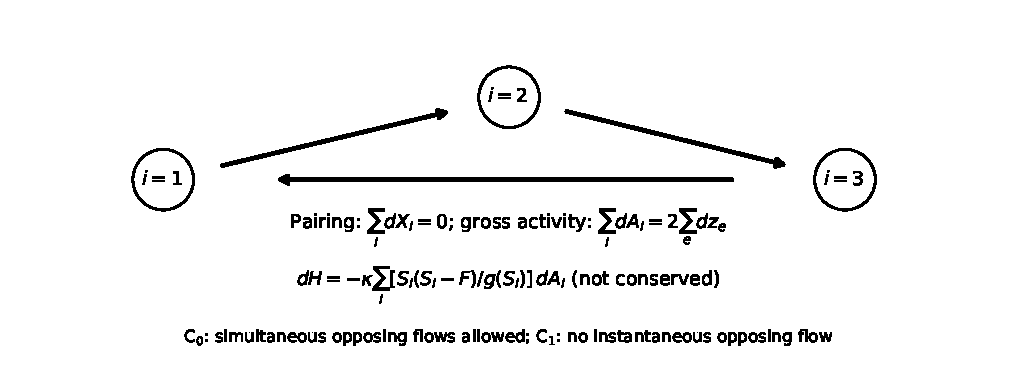
\includegraphics[width=.87\linewidth]{figures/Fig01_trade_activity_not_conservation.pdf}
\caption{Paired executed-dollar transfers and positive gross activity.
The activity-driven potential is not generally conserved. This
replaces the old physical-time conservation diagram.}
\label{fig:activity}
\end{figure}

\begin{figure}[tb]
\centering
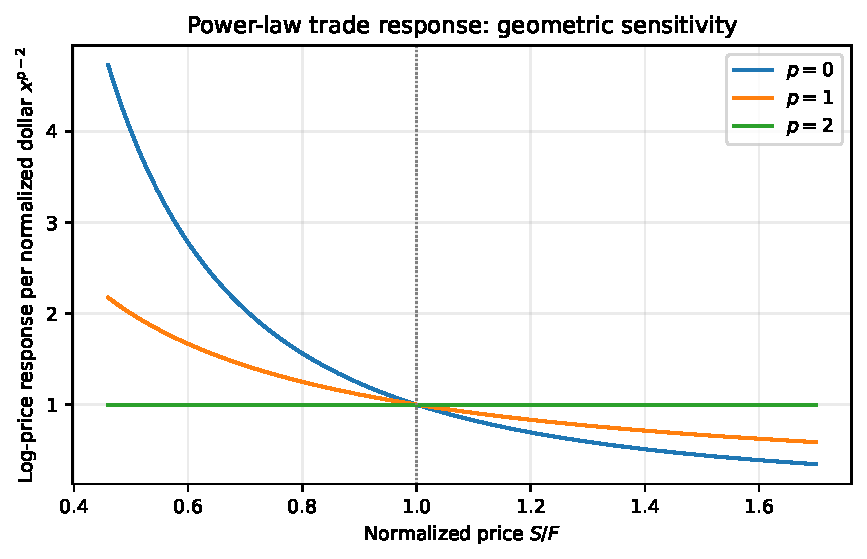
\includegraphics[width=.87\linewidth]{figures/Fig02_powerlaw_log_response.pdf}
\caption{Power-law response and normalized log sensitivity in the
new model. Curves illustrate scalar mechanisms; they do not
constitute a complete global $(p,K,N)$ reachability phase diagram.}
\label{fig:response}
\end{figure}

\begin{figure}[tb]
\centering
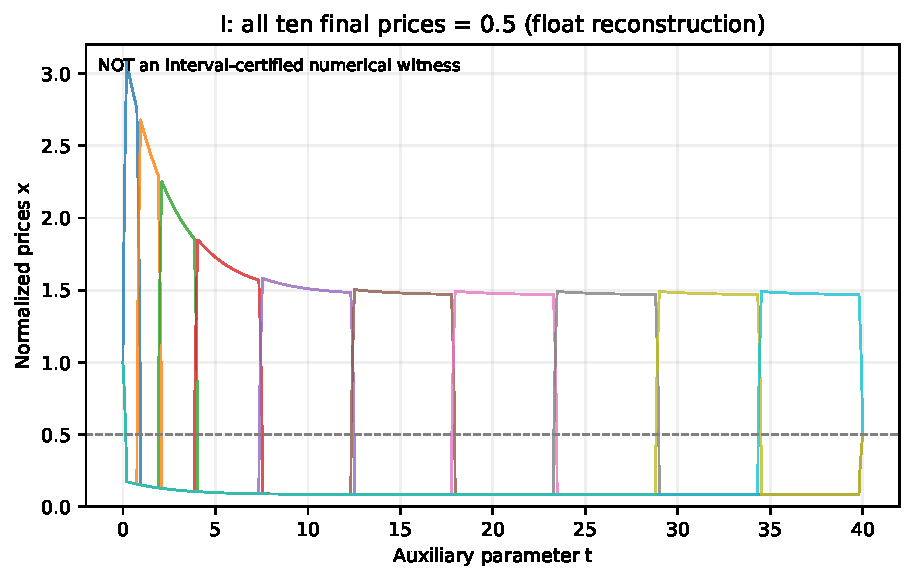
\includegraphics[width=.86\linewidth]{figures/Fig03_I_ten_asset_float_paths.pdf}
\caption{Ten-asset half-price trajectory from the independent
\emph{floating-point} trial with $K=1/75$, $T=40$, $M=6000$.
The exact analytic witness of Theorem~\ref{thm:tenhalf} uses
different parameters and does not certify this plotted root.}
\label{fig:ten-trial}
\end{figure}

\begin{figure}[tb]
\centering
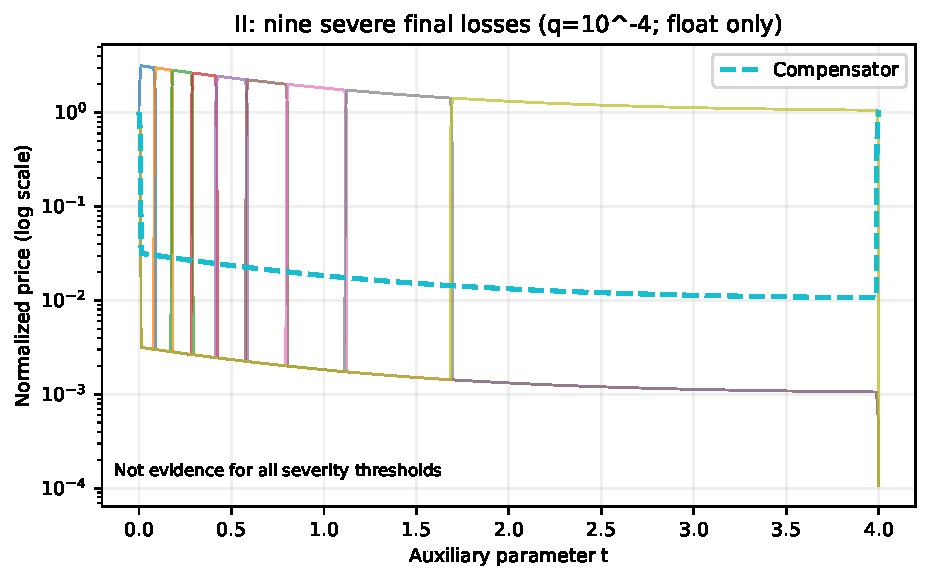
\includegraphics[width=.86\linewidth]{figures/Fig04_II_nine_target_float_paths.pdf}
\caption{Nine-target severe-loss trial using $T=4$, $K=.002$,
$M=10000$, based on a floating-point reconstruction. Extreme
$q$ inventory quadrature is not reported as precisely known.}
\label{fig:nine-trial}
\end{figure}

\begin{table}[tb]
\centering\small
\caption{Guaranteed severity levels from the \emph{analytic} family
of Theorem~\ref{thm:nine}. For each row take
$q_\delta=e^{-2\delta-5}\le0.01$. These are exact existence
bounds, \emph{not} reconstructions of the floating-point trial roots.}
\label{tab:analytic-severity}
\begin{tabular}{@{}ccccc@{}}\toprule
Target $\delta$ & Terminal direction $q_\delta$ & Guaranteed
$\Cris_{0.9}(T)$ & $M$ & $\max_i H_i^-$ \\\midrule
$3$ & $e^{-11}$ & $>3$ & $10^{20}$ & $<3\cdot10^{24}$\\
$5$ & $e^{-15}$ & $>5$ & $10^{20}$ & $<3\cdot10^{24}$\\
$10$ & $e^{-25}$ & $>10$ & $10^{20}$ & $<3\cdot10^{24}$\\
$20$ & $e^{-45}$ & $>20$ & $10^{20}$ & $<3\cdot10^{24}$\\\bottomrule
\end{tabular}
\end{table}
The guarantee uses only $1\le R(T)<4$ and
$x_i(T)=q_\delta R(T)$ for nine targets: their log losses
exceed $2\delta+5-\log4$, while the compensator's log loss
exceeds $-\log4$. Hence
\[
 \Cris_{0.9}(T)\ge\min\!\left\{
 2\delta+5-\log4,\,
 \frac{9(2\delta+5-\log4)-\log4}{10}\right\}>\delta.
\]
This table restores the original severity-ladder question with a
proved bound rather than claiming that an approximate trajectory
attains a certified terminal price.

\begin{table}[tb]
\centering\small
\caption{Reconstruction of the old activity-model \emph{numerical trials}.
Numbers are floating-point estimates, not exact root certificates.
The $q=10^{-8}$ share total is intentionally omitted because
quadrature was not stable. This table is not the analytic severity
menu in Table~\ref{tab:analytic-severity}.}
\label{tab:reconstruction}
\begin{tabular}{@{}lrrrl@{}}\toprule
Trial & $M$ & $\Cris_{0.9}(T)$ & Max ledger residual & Gross shares \\\midrule
I, ten halves & $6000$ & --- & $1.03\cdot10^{-9}$ & $6724.54$ (max)\\
II, $q=10^{-2}$ & $10000$ & $4.08329$ & $2.16\cdot10^{-10}$ & $698769.15$ (max)\\
II, $q=10^{-4}$ & $10000$ & $8.22846$ & $2.16\cdot10^{-10}$ & $703402.95$ (max)\\
II, $q=10^{-8}$ & $10000$ & $16.51777$ & $1.25\cdot10^{-10}$ & not reliably integrated \\\bottomrule
\end{tabular}
\end{table}

\begin{figure}[tb]
\centering
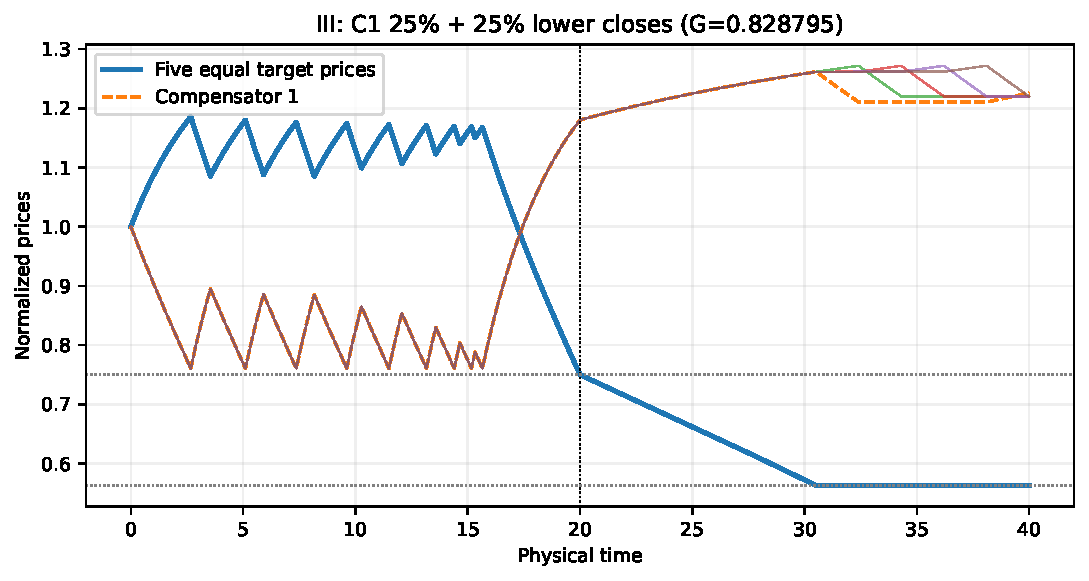
\includegraphics[width=.87\linewidth]{figures/Fig05_III_C1_two_session_prices.pdf}
\caption{Two-session target and compensator prices for the
$\mathsf C_1$ five-target construction. Root isolation and path
bounds are derived from interval enclosures, not the pixels.}
\label{fig:twosession}
\end{figure}

\begin{figure}[tb]
\centering
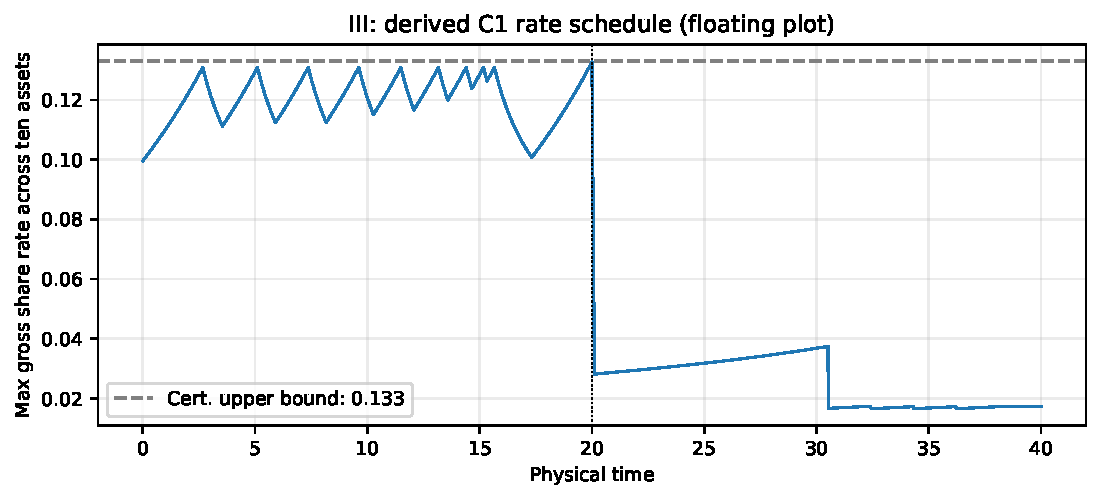
\includegraphics[width=.87\linewidth]{figures/Fig06_III_C1_max_gross_share_rate.pdf}
\caption{Gross executed-share-rate schedule for the certified
rolling-band construction. The per-node maximum is less than
$.133$ in the specified time allocation.}
\label{fig:grossrate}
\end{figure}

\FloatBarrier

\section{Conditional robustness and heterogeneous quadratic response}
\label{sec:robustness}
The following two modifications of the base law are \emph{separate
models}. They are included to identify which structural barriers use
homogeneous response and exactly paired execution. They are not silent
extensions of the admissible control set in Definition~\ref{def:controls}.

\begin{proposition}[Unpaired forcing: continuous dependence and closure]
\label{prop:unmatched}
Consider the formal perturbation
\begin{equation}\label{eq:unmatched}
 \dd X_i=\sum_e B_{ie}\,\dd z_e+e_i(t)\dd t,
 \qquad\dd A_i=\sum_e|B_{ie}|\,\dd z_e,
 \qquad e_i\in L^1(0,T).
\end{equation}
The additional forcing is \emph{not} itself counted as a real matched
transaction or as gross executed-dollar activity. Let $S^e,S^0$ be
solutions with the same nonnegative paired-edge flows, parameters and
initial prices, with $e$ and $0$ respectively. Suppose both paths stay
in a common positive compact price interval $I=[m,U]$. Put
$y=\Phi(S)$ and let $L$ be a Lipschitz constant of
$R\circ\Phi^{-1}$ on $\Phi(I)$, and
$G=\sup_{S\in I}g(S)/S$. Then
\begin{align}
 \sup_{0\le t\le T}|y_i^e(t)-y_i^0(t)|
 &\le e^{\kappa L A_i(T)}\,\|e_i\|_{L^1(0,T)},\label{eq:robust}\\
 \sup_{0\le t\le T}|S_i^e(t)-S_i^0(t)|
 &\le G e^{\kappa L A_i(T)}\,\|e_i\|_{L^1(0,T)}.
 \label{eq:price-robust}
\end{align}
In particular, for each $\alpha\in(0,1]$,
\begin{equation}\label{eq:crisis-robust}
 |\Cris_\alpha^e(T)-\Cris_\alpha^0(T)|
 \le \frac{G}{m}\max_i
 \left[e^{\kappa L A_i(T)}\|e_i\|_{L^1(0,T)}\right].
\end{equation}
If the baseline ledger is terminally closed and
$\int_0^T e_i(t)\dd t=0$ for each asset, the perturbed ledger is
also terminally closed. In the absence of this \emph{separate}
zero-integral condition, terminal closure is not preserved in general.
\end{proposition}
\begin{proof}
In the transformed coordinate, the paired flow term is identical
for the two trajectories, and
$\dd(y_i^e-y_i^0)=e_i(t)\dd t
-\kappa\{R(S_i^e)-R(S_i^0)\}\dd A_i$.
Gronwall's inequality in the nonnegative activity measure gives
the first estimate. Since
$(\Phi^{-1})'(y)=g(S)/S\le G$ on the stipulated strip,
the second follows. The scalar loss function $S\mapsto\log(F/S)$
is $1/m$-Lipschitz on $I$. Its arithmetic mean and its
$k$th-largest order statistic are each 1-Lipschitz in the sup norm
of the vector of losses, as is their minimum. This proves
\eqref{eq:crisis-robust}. Finally, integrate \eqref{eq:unmatched}:
$X_i^e(T)-X_i^0(T)=\int_0^T e_i(t)\dd t$.
\end{proof}

\begin{proposition}[Heterogeneous quadratic response: exact weighted balance]
\label{prop:hetero-weighted}
Fix a common fundamental level $F>0$. At node $i$ let
$g_i(S)=\eta_i(S/F)^2$ and $\kappa_i>0$, with
$D_i=F^2/\eta_i>0$ and $q_i=\log(S_i/F)$. Use actual paired-dollar
flows and the activity law \eqref{eq:model}, allowing $\eta_i$ and
$\kappa_i$ to differ between assets. Then every flow-completed path
satisfies the \emph{exact} relations
\begin{align}
 D_i\dd q_i&=\dd X_i-\kappa_iD_i(1-e^{-q_i})\dd A_i,
 \label{eq:hetero-node}\\
 \dd\Bigl(\sum_i D_i q_i\Bigr)
 &=-\sum_i\kappa_iD_i(1-e^{-q_i})\dd A_i.
 \label{eq:hetero-balance}
\end{align}
More generally, for arbitrary fixed weights $w_i$,
\begin{equation}\label{eq:hetero-imbalance}
 \dd\Bigl(\sum_iw_iq_i\Bigr)
 =\sum_e\Bigl(\frac{w_{b(e)}}{D_{b(e)}}
                  -\frac{w_{s(e)}}{D_{s(e)}}\Bigr)\dd z_e
 -\sum_i w_i\kappa_i(1-e^{-q_i})\dd A_i.
\end{equation}
If a path is bounded above by $S_i(t)\le U_i$ and
$A_i^+=\int_{S_i>F}\dd A_i$, set
$\chi_i^+=\pos{1-F/U_i}$. Then
\begin{equation}\label{eq:hetero-high}
 \sum_iD_iq_i(T)\ge
 -\sum_i\kappa_iD_i\chi_i^+A_i^+.
\end{equation}
Consequently, if all assets end below their benchmarks with
$q_i(T)\le-\delta_i$ and $\delta_i\ge0$, a necessary condition is
\begin{equation}\label{eq:hetero-resource}
 \sum_iD_i\delta_i
 \le\sum_i\kappa_iD_i\chi_i^+A_i^+.
\end{equation}
The inequalities are \emph{necessary}, and they do not certify an
unweighted systemic crisis or a globally sharp turnover bound.
\end{proposition}
\begin{proof}
For $g_i(S)=\eta_i(S/F)^2$,
$\Phi_i(S)=D_i\log(S/F)$ and
$R_i(S)=D_i(1-F/S)$. Apply the chain rule to every
completed edge and use $\sum_i\dd X_i=0$. Keeping the
weighted incidence term rather than cancelling it gives
\eqref{eq:hetero-imbalance}. Where $S_i\le F$,
$1-F/S_i\le0$, so these contributions are nonnegative in
\eqref{eq:hetero-balance}; where $S_i>F$ they are bounded
above by $\chi_i^+$. This yields \eqref{eq:hetero-high} and
then \eqref{eq:hetero-resource}.
\end{proof}

\begin{proposition}[A closed-dollar two-node quadratic counterexample]
\label{prop:hetero-two}
Consider two assets in the heterogeneous quadratic model, with
$\kappa_1/D_1>\kappa_2/D_2>0$. Execute one dollar transfer
of amount $z$ from asset $2$ to asset $1$, followed immediately
in \emph{activity order} by the reverse transfer of the same
amount $z$. The completed-event trajectory belongs to
$\mathsf C_1$, remains strictly positive for sufficiently small
$z>0$, and satisfies $X_1(T)=X_2(T)=0$. Nevertheless
\begin{equation}\label{eq:hetero-two-loss}
 \overline L(T)=\frac12\Bigl(\frac{\kappa_1}{D_1}
                 -\frac{\kappa_2}{D_2}\Bigr)z^2+O(z^3)>0,
 \qquad Q_{1/2}(T)>0.
\end{equation}
Thus $\Cris_{1/2}(T)>0$ although both response elasticities
equal two. This does \emph{not} contradict the homogeneous
common-clock barrier in Proposition~\ref{prop:two-node-barriers};
its common-parameter assumption is essential.
\end{proposition}
\begin{proof}
During an edge of dollar amount $a$, with incidence sign
$\sigma_i\in\{-1,1\}$, the log price satisfies
\begin{equation}\label{eq:hetero-edge}
 \frac{\dd q_i}{\dd a}=\frac{\sigma_i}{D_i}
             -\kappa_i(1-e^{-q_i}).
\end{equation}
The leading log-price path is the triangle
$q_i^{(0)}(a)=\sigma_i a/D_i$ for $0\le a\le z$ and
$q_i^{(0)}(a)=\sigma_i(2z-a)/D_i$ for $z\le a\le2z$.
Its integral is $\sigma_i z^2/D_i$. Since
$1-e^{-q}=q+O(q^2)$ uniformly for $|q|=O(z)$, and
$\int_0^{2z}\sigma_i\dd a=0$, integration of
\eqref{eq:hetero-edge} gives
$q_i(2z)=-\sigma_i\kappa_i z^2/D_i+O(z^3)$.
Take $\sigma_1=+1$, $\sigma_2=-1$. The first log price is
negative, the second positive, and their arithmetic mean is
negative precisely under the assumed coefficient inequality.
True gross seller-side share quantities are finite because the
entire path stays in a compact positive neighborhood of $F$.
\end{proof}

The results in this section distinguish exact changes in the model
from robustness within it. Formula \eqref{eq:robust} is a
\emph{conditional} comparison for fixed edge flows, not a
control perturbation theorem preserving exact target prices. The
heterogeneous weighted identity does not supply a new
unweighted global phase diagram. In particular, global large-turnover
two-asset reachability for homogeneous $1<p<2$, sharp full-coverage
severity, maximum repeated-limit breadth, and globally optimal
execution rates remain open.

\section{Interpretation and limitations}\label{sec:discussion}
The activity clock breaks the trade-time conservation of
$\sum_i\Phi(S_i)$. Its rate is instead
$-\kappa\sum_iR(S_i)\dd A_i$; the sign depends on the placement
of gross activity across price regions. The local triangular protocol
is already available in $\mathsf C_1$, but the large existence
constructions I--II exploit the broader $\mathsf C_0$ by assigning
common activity even to nodes with small net dollar rates. Such
churning is real executed dollar volume under the stipulated control
rules, not a claim about rational investors' equilibrium behavior.
The $\mathsf C_1$ two-session construction excludes instantaneous
netting but uses many temporal direction reversals; prohibiting
round trips altogether is a different admissibility restriction.

Proposition~\ref{prop:hetero-two} shows that even the
two-node quadratic-response obstruction is parameter-sensitive:
heterogeneous activity-recovery coefficients permit a
closed-dollar local systemic loss. Theorem~\ref{thm:two-large-turnover}
adds a complementary homogeneous result: throughout
$1<p\le3/2$, a finite turnover path achieves a two-node
systemic loss despite the rigorous small-turnover barrier.
The explicit $p=5/4$ witness obeys the stricter
$\mathsf C_1$ constraint and a finite gross share-rate cap.
Corollary~\ref{cor:nearcritical-beyond} additionally
proves a nonempty reachable interval immediately above
$p=3/2$ for every fixed $K$. The global classification
outside this demonstrated range remains open; none of
these results introduces strategic trading incentives.

For $p<1$ the scalar floor boundary $K_c(p)$ rules out
unbounded severity at sufficiently large $K$, while
Theorem~\ref{thm:nine-general} establishes a nonempty
fixed-exponent existence region (with explicit $p=0$ constants
in Theorem~\ref{thm:nine}).
The intervening parameter range and sharp resource-efficient bounds
remain open. Price-floor nonexistence alone is not a sufficiency
theorem. The two-session witness establishes attainability for
\emph{five} targets. Corollary~\ref{cor:at-most-n-minus-one}
rules out simultaneous repeated lower closes for all ten,
so the attainable optimum is between five and nine. The
former seven-target obstruction of the physical-time model
is not transferred here.

\section{Conclusion}
In an idealized fixed-benchmark market where every dollar transfer
is paired and every asset's terminal dollar ledger closes, gross
trade activity can induce both price impact and resilience.
Three-asset trading cycles yield local all-market losses, while
scalar floors, aggregate barriers and necessary execution bounds
restrict their scale. In the quadratic family, the exact heterogeneous
weighted balance and a two-node round-trip counterexample delimit
the homogeneous barrier. Exact analytic continuation establishes
all-ten halving and, for each fixed $0\le p<1$, a nine-target
uniform-resource severity family;
an independent internally certified ten-asset control achieves
five repeated lower-limit closes with finite rate and strict
sessionwise bands. These conclusions concern deterministic
admissibility, not real-world crash probability or strategic
profitability.

\appendix

\section{One-sided bounded variation and true seller-side inventory}
\label{app:bv}
This appendix proves the low-price variation statement used in
Theorem~\ref{thm:lower} without reusing the physical-time
restoration estimates of the earlier model.

\begin{lemma}[Low-price excursion and one-sided variation]
\label{lem:one-sided-bv}
Let $S_i:[0,T]\to(0,\infty)$ be a continuous,
flow-completed, finite-variation price path with $S_i(0)=F$,
$\kappa>0$ and $g>0$. Define the cumulative \emph{net} share
ledger $\theta_i$ by $\dd\theta_i=\dd X_i/S_i$, and let
$\operatorname{Var}^-(Z;[0,T])$ denote the negative Jordan
variation of a continuous finite-variation path $Z$. Then
\begin{align}
 \pos{-\Phi(S_i(T))}
 &\le\operatorname{Var}^-(X_i;[0,T]),
 \label{eq:var-dollar}\\
 \pos{-\Psi(S_i(T))}
 &\le\operatorname{Var}^-(\theta_i;[0,T])
 \le H_i^-.
 \label{eq:var-shares}
\end{align}
In the broader control class $\mathsf C_0$ the final two
quantities need \emph{not} be equal; simultaneous genuine buys
and sells increase gross shares even when net share flow cancels.
\end{lemma}
\begin{proof}
The inequalities are void if $S_i(T)\ge F$. Otherwise let
$t_*\in[0,T)$ be the last time $S_i(t_*)=F$; continuity and
$S_i(0)=F$ guarantee such a time. Then $S_i(t)<F$ for
$t\in(t_*,T]$. On this interval, $R(S_i)\le0$, hence
\[
 \dd\Phi(S_i)=\dd X_i-\kappa R(S_i)\dd A_i\ge\dd X_i.
\]
Integration from $t_*$ to $T$ gives
$X_i(T)-X_i(t_*)\le\Phi(S_i(T))<0$, and the negative
variation of $X_i$ dominates the absolute value of that
negative net increment. Similarly, since
$\Psi'(S)=1/g(S)$,
\[
 \dd\Psi(S_i)=\dd\theta_i
       -\kappa\frac{S_i-F}{g(S_i)}\dd A_i\ge\dd\theta_i
\]
on the same final excursion. This proves the first inequality
in \eqref{eq:var-shares}. On every event, the negative part of
$\dd\theta_i$ is bounded by the sum of shares actually sold,
$\sum_{e:B_{ie}=-1}\dd z_e/S_i$. Integrate this pointwise
measure domination to obtain
$\operatorname{Var}^-(\theta_i)\le H_i^-$. The reasoning
also applies to arbitrary absolutely continuous simultaneous
$\mathsf C_0$ edge flows; no invalid cancellation of gross
trades was made.
\end{proof}

For a terminal price $S_i(T)\le s<F$, monotonicity of
$\Phi$ and $\Psi$ gives
$\operatorname{Var}^-(X_i)\ge-\Phi(s)$ and
$H_i^-\ge-\Psi(s)$. Sum these bounds over any $k$ target
assets. For the dollars, seller-side negative variation is
bounded by actual seller-side dollar flow, which counts
\emph{each paired edge exactly once}. This produces
\eqref{eq:bounds}; it is a necessary market-resource bound,
not an existence statement.

\section{Gross-share execution rates: explicit bootstrap and a matching local order}
\label{app:rates}
The following proof gives a rate constant that does not depend
on a selected small rate $v$, provided the local condition is
formulated with a fixed strip margin. It also makes precise the
claim of local quadratic order in $\mathsf C_1$.

\begin{proposition}[Uniform small-rate bound with a fixed strip]
\label{prop:rate-explicit}
Let $I=[F-d,F+d]$ with $0<d<F$, and set
$h(S)=g(S)/S$ and $C_I,U_I,L_I$ as in
Theorem~\ref{thm:ratequadratic}. If
\begin{equation}\label{eq:rate-small}
 v C_I T<\min\{d,F/2\},
\end{equation}
then every admissible paired execution satisfying
$\dot A_i/S_i\le v$ stays in $I$ and obeys the explicit bound
\begin{equation}\label{eq:rate-B}
 \Cris_\alpha(T)\le\bar L(T)\le
 \left\{\frac{C_IU_I(L_I+\kappa)}{2F}
           +\frac{2C_I^2}{F^2}\right\}v^2T^2.
\end{equation}
The constant in braces is independent of $v,T$, although it
depends on the fixed price strip and response parameters.
\end{proposition}
\begin{proof}
On any subinterval before the first exit from $I$,
\[
 |\dot S_i|\le h(S_i)|\dot X_i|
               +\kappa|S_i-F|\dot A_i
 \le v\{g(S_i)+\kappa S_i|S_i-F|\}\le v C_I.
\]
Thus $|S_i(t)-F|\le v C_I t<d$, excluding a first exit.
Let $y_i=S_i-F$. Since $\sum_i\dot X_i=0$ and
$|\dot X_i|\le\dot A_i\le vU_I$,
\[
 \left|\frac{\dd}{\dd t}\bar S(t)\right|
 \le\frac1N\sum_i
 \Bigl\{L_I|y_i|\,|\dot X_i|
             +\kappa|y_i|\dot A_i\Bigr\}
 \le v^2 C_I U_I(L_I+\kappa)t.
\]
After integration,
$|\bar S(T)-F|\le\tfrac12v^2T^2C_IU_I(L_I+\kappa)$.
For $|w|\le\tfrac12$, Taylor's inequality
$-\log(1+w)\le-w+2w^2$ gives, with $w_i=y_i/F$,
\[
 \bar L(T)\le-\frac{\bar S(T)-F}{F}
     +\frac{2}{NF^2}\sum_i y_i(T)^2.
\]
The already proved $|y_i(T)|\le vC_IT<F/2$
then yields \eqref{eq:rate-B}.
\end{proof}

\begin{proposition}[Time-resolved $\mathsf C_1$ triangle attains quadratic order]
\label{prop:rate-local-match}
Fix $N\ge3$, a common positive $C^2$ response $g$, and
$\kappa>0$. There are constants $\varepsilon,C_1,C_2>0$,
depending on $N,F,g,\kappa$, such that for every
$0<vT<\varepsilon$ one can construct a dollar-closed
$\mathsf C_1$ path on $[0,T]$ whose true gross share rate
satisfies $\sup_{i,t}\dot A_i/S_i\le v$ and whose terminal
systemic loss obeys
\begin{equation}\label{eq:rate-match}
 \Cris_1(T)\ge C_1(vT)^2>0,
 \qquad M\le C_2 vT.
\end{equation}
Thus, for fixed $N$ and a small local rate--horizon product,
the quadratic scaling exponent of
Proposition~\ref{prop:rate-explicit} cannot in general be
improved to a higher power.
\end{proposition}
\begin{proof}
Take the nine-edge triangle from
Theorem~\ref{thm:triangle} for nodes $(1,2,3)$. For
$N>3$, concatenate one triangle on $(1,2,j)$ for each
$j=4,\ldots,N$; for $N=3$ use only the first triangle.
Let $m=9\max\{1,N-2\}$ be the total number of edges and
assign each edge a dollar amount $z>0$ and a time interval
of length $T/m$. Each active edge then has dollar rate
$mz/T$, and only its buyer and seller have positive gross
activity. For sufficiently small $z$, all prices stay within
$[F/2,3F/2]$. Therefore the gross share rate is bounded by
$2mz/(FT)$. Choose $z=FvT/(4m)$; the rate is at most
$v/2$, with a strict margin for all sufficiently small $vT$.
The nine-edge expansion establishes that at the end of each
triangle its three participating nodes undergo a strictly
negative transformed-price change of magnitude
$\kappa z^2$ times a fixed positive response-dependent
coefficient, with an $O(z^3)$ remainder. The triangles
start at prices $F+O(z^2)$, so composition retains a negative
$-c_i z^2+O(z^3)$ leading term at every node, with
$c_i>0$ depending on its number of triangle memberships.
The mean terminal log loss and every individual log loss
are therefore bounded below by $C z^2$ for some fixed
$C>0$ once $z$ is sufficiently small. Thus
$\Cris_1\ge C z^2=C_1(vT)^2$.
Every dollar edge is paired, no asset buys and sells at the same
instant, and its incident amounts comprise equal purchases and
sales over each completed triangle; all net-dollar ledgers close
exactly. The paired turnover is $M=m z=(F/4)vT$.
\end{proof}

\section{Quantitative cut-root existence and constant-resource construction}
\label{app:smoothing}
This appendix records the derivatives and numerical inequalities
supporting Theorems~\ref{thm:tenhalf} and \ref{thm:nine}.
They do \emph{not} certify the cached floating-point roots.

\subsection{Exact activity-driven radial identity}
Let $Y_i(t)>0$, $\sum_iY_i(t)=1$, and $x_i=R\sqrt{Y_i}$.
If
\begin{equation}\label{eq:radial}
 R'=\rho(H(Y)-R),\quad H(Y)=\sum_i\sqrt{Y_i},\quad
 R(0)=\sqrt{10},
\end{equation}
and
\begin{equation}\label{eq:rateformula}
 u_i=\frac{R^2}{2}Y_i'
    +\rho R\bigl(H(Y)Y_i-\sqrt{Y_i}\bigr),
\end{equation}
then $\sum_i u_i=0$ and
$\dot x_i=u_i/x_i-\rho(x_i-1)$. Taking equal constant gross
dollar activity $\dot a_i=a_0$, $K=\rho/a_0$, makes these
the original \emph{activity-driven} dynamics, not an external
time-decay approximation. Chain rule gives the exact terminal
ledger, with $\psi(z)=z(z-1)$,
\begin{equation}\label{eq:ledgerradial}
 X_i(T)=\frac{R(T)^2Y_i(T)-1}{2}
             +\rho\int_0^T\psi(R(t)\sqrt{Y_i(t)})\,dt.
\end{equation}
Since $1\le H(Y)\le\sqrt{10}$, the solution to
\eqref{eq:radial} satisfies $1\le R\le\sqrt{10}$.

\subsection{Exact Green inverse for cut times}
On each of $m$ constant-direction role stages, the radial source
$H_b$ is the same because the role directions differ by
permutation only. Write
$A_j=\int_{t_{j-1}}^{t_j}W_b(t)dt$,
where $W_b$ is the positive high-minus-low ledger integrand.
Equating adjacent account ledgers yields
$D_j=\rho(A_j-A_{j+1})=0$ for $j=1,\dots,m-1$.
The sharp Jacobian is
\begin{equation}\label{eq:sharpJ}
 J_0=\rho L_{m-1}\operatorname{diag}(W_b(t_1),\dots,W_b(t_{m-1})),
\end{equation}
with $L_n$ the Dirichlet tridiagonal matrix $2,-1,-1$.
Its inverse admits an \emph{exact} discrete Green kernel:
\[
 (L_{m-1}^{-1})_{ij}=
 \frac{\min(i,j)(m-\max(i,j))}{m},
 \qquad \|L_{m-1}^{-1}\|_\infty
 =\max_i\frac{i(m-i)}2.
\]
Consequently the inverse norms are $25/2$ for ten stages
and $10$ for nine. If $W_b\ge w_*>0$, then
$\|J_0^{-1}\|_\infty\le\|L^{-1}\|_\infty/(\rho w_*)$,
and $\det J_0=m\rho^{m-1}\prod_jW_b(t_j)>0$.
This is a quantitative nondegeneracy certificate; it does not
assert that a double-precision cut vector is a mathematical root.

\subsection{Moving ramps: correct $L^1$, not $L^\infty$, derivative}
Take an interior $h$-wide affine $Y$-ramp centered at a cut $\tau$.
The two flanking role stages have the \emph{same} source $H_b$,
and the ramp contributes a compact pulse
$\Delta_h(t;\tau)=d_b((t-\tau)/h)$ with
$\Delta_h=0$ at both endpoints and
$|\Delta_h|\le D_*\le4$. Differentiation of the radial
variation-of-constants formula followed by integration by parts
gives the exact identity
\begin{equation}\label{eq:movingderivative}
 \partial_\tau R_h(t)=-\rho\Delta_h(t;\tau)
 +\rho^2\int_0^t e^{-\rho(t-s)}\Delta_h(s;\tau)ds.
\end{equation}
The right-hand side is $O(1)$ \emph{inside} the ramp, so a
pointwise global $O(h)$ derivative estimate would be false.
However, Tonelli's theorem yields
\begin{equation}\label{eq:movingsensitivity}
 \|\partial_\tau R_h\|_{L^1(0,T)}\le2\rho D_*h,
 \qquad |\partial_\tau R_h(T)|\le\rho^2D_*h.
\end{equation}
The integrand in \eqref{eq:ledgerradial} has bounded radial
derivative $|\partial_R\psi(R\sqrt{Y_i})|\le9$.
The integrated radial part of the cut derivative is therefore
$O(h)$. The direct interpolation derivative converges to the
jump between adjacent sharp-stage integrands, uniformly over
compact positive internal direction parameters. The end ramps
are stationary when interior cuts vary. In Construction II the
terminal direction $q\downarrow0$ is included only as a
continuous endpoint parameter, never differentiated with
respect to $q$ at zero.

\subsection{Explicit contraction and sign bounds}
Choose $h=10^{-16}$, a cut-neighborhood radius $r=10^{-6}$ and
$a_0=10^{17}$. For Construction I, the compact parameter interval
$b\in[3/50,7/100]$ has $W_b>.7$ and ten sharp stage gaps
larger than $14/65$. The endpoint residual
$R_b(40)/\sqrt{10}-1/2$ is below $-.018$ on the left and
above $.001$ on the right. There are eleven smoothing windows;
from their total length and $1\le R\le\sqrt{10}$,
\[
 \|R_h-R_b\|_\infty<18h,\quad
 \max_i|X_i^h-X_i^0|<2800h,\quad
 \max_{i,j}|\partial_{t_j}X_i^h-
                    \partial_{t_j}X_i^0|<200h.
\]
The $\infty$-norm Jacobian preconditioner is below $45$,
so the contraction norm is smaller than
$45[(2/5)400r+3600h]<1/4$ and center displacement is
below $45(2\cdot2800h)<r/2$.
The resulting exact cut roots preserve the endpoint signs.

For Construction II, take
$b\in[10^{-5},.05]$, $c=.01$, $T=200$.
The sharp compensator ledger is greater than $.06$ at the left
endpoint and less than $-3$ at the right for all
$0\le q\le.01$. The weight satisfies $W_b>.08$ and
nine stage gaps exceed $16/117$. The ten smoothing windows give
\[
 \|R_h-R_b\|_\infty\le40h,\quad
 \max_i|X_i^h-X_i^0|\le72400h,\quad
 \max_{i,j}|\partial_{t_j}X_i^h-
                    \partial_{t_j}X_i^0|<1000h.
\]
With $\|J_0^{-1}\|_\infty\le125$, the contraction norm is
$125(400r+16000h)<1/4$ and the center displacement
is $125(2\cdot72400h)<r/2$. These statements apply
\emph{uniformly in $q$}, with one fixed strictly positive $h$.
The exact rational inequalities, including square-root and
exponential brackets, are also checked by the independent
\texttt{certify\_gate2\_explicit.py} diagnostic; the script
is not a substitute for the analytic derivation.

\subsection{Edge completion, finite turnover, and true gross inventories}
Equation \eqref{eq:rateformula} implies
$|u_i|\le5/h+8$ for I and $|u_i|\le5/h+20$ for II,
which are both below $a_0=10^{17}$. At each instant prescribe
purchases $b_i=(a_0+u_i)/2$ and sales $s_i=(a_0-u_i)/2$.
The complete directed graph without self-edges admits a
nonnegative transportation matrix from the sellers to the
buyers because total supplies and demands both equal
$Na_0/2$ and every singleton satisfies
$b_i+s_i=a_0\le Na_0/2$.
Thus $A_i'=a_0$, $X_i'=u_i$ and
$M=Na_0T/2$, \emph{with real gross opposite flows} in
$\mathsf C_0$ rather than a fictitious ``activity clock.''
In I, every price remains above $.06$, giving
$H_i^-<a_0T/.06<10^{20}$. In II, before the final ramp every
price is at least $10^{-5}$; on the last ramp target prices are
at least $c\sqrt{1-s}$ for $0\le s\le1$. Therefore
$\int_{T-h}^T dt/x_i\le2h/c$, independent of $q>0$;
this leads to $H_i^-<3\cdot10^{24}$.
No fixed \emph{pointwise} share-rate cap is claimed for II as
$q\downarrow0$.

\section{The sublinear-exponent radial representation and its uniform inventory lemma}
\label{app:general-p}
This section makes explicit the scope of the fixed $p<1$
research extension. It establishes the change of variables and
the \emph{resource integrability} at a terminal zero-direction
limit, but the sharp-cut bracketing and Jacobian estimates
are proved below for each fixed exponent; the $p=0$ certificate
is not a universal numerical certificate in $p$.

\begin{lemma}[Exact radial identities for $0\le p<1$]
\label{lem:radial-general}
Let $\nu=2-p>1$, normalize $F=\eta=1$, and prescribe
identical gross dollar-activity rates $\dot a_i=a_0$ with
$\rho=Ka_0$. For a continuously differentiable path of
strictly positive directions $Y_i(t)$ with $\sum_iY_i=1$,
set $x_i=R Y_i^{1/\nu}$. Then the paired-dollar balance
$\sum_i\dot u_i=0$ holds precisely when
\begin{equation}\label{eq:radial-general}
 R'=\rho\{H_\nu(Y)-R\},\qquad
 H_\nu(Y)=\sum_iY_i^{(\nu-1)/\nu}.
\end{equation}
For that radial solution the required net-dollar rates are
\begin{equation}\label{eq:controls-general}
 \dot u_i=\frac{R^\nu}{\nu}\dot Y_i
   +\rho R^{\nu-1}\left\{H_\nu(Y)Y_i
                               -Y_i^{(\nu-1)/\nu}\right\},
\end{equation}
and each terminal ledger satisfies
\begin{equation}\label{eq:ledger-general}
 u_i(T)=\frac{x_i(T)^\nu-1}{\nu}
  +\rho\int_0^T x_i(t)^{\nu-1}\{x_i(t)-1\}\dd t.
\end{equation}
In particular, with $R(0)=N^{1/\nu}$ and
$Y_i(0)=1/N$, the radial solution remains in the strip
$1\le R(t)\le N^{1/\nu}$.
\end{lemma}
\begin{proof}
Differentiation of $x_i^\nu$ in the normalized activity
law gives
$\frac1\nu\frac\dd{\dd t}x_i^\nu
=\dot u_i-\rho x_i^{\nu-1}(x_i-1)$.
Sum over all assets and use the zero-sum net-dollar rates.
Since $\sum_i x_i^\nu=R^\nu$ and
$\sum_i x_i^{\nu-1}=R^{\nu-1}H_\nu(Y)$,
the equation for $R$ follows. Solving the individual
identity for $\dot u_i$ and substituting
\eqref{eq:radial-general} yields
\eqref{eq:controls-general}; its components sum to zero.
Integration gives \eqref{eq:ledger-general}, since
$u_i(0)=0$ and $x_i(0)=1$.
Finally, Holder's inequality and concavity give
$1\le H_\nu(Y)\le N^{1/\nu}$ for $Y_i\ge0$ on the
simplex. Scalar comparison proves the asserted radial bounds.
\end{proof}

\begin{lemma}[Uniform terminal share integrability]
\label{lem:terminal-inventory}
Suppose that on a final window $[T-h,T]$, with
$0<h<\infty$ fixed, each target direction follows an affine
path from a positive fraction at least $c^\nu$ to a terminal
fraction $q^\nu$, where $c>0$ and $0<q<c$. Put
$s=(t-T+h)/h\in[0,1]$. Then
\begin{equation}\label{eq:inventory-general}
 Y_i(t)\ge c^\nu(1-s),\qquad
 x_i(t)\ge c(1-s)^{1/\nu},\qquad
 \int_{T-h}^T\frac{\dd t}{x_i(t)}
 \le\frac{h\nu}{c(\nu-1)}.
\end{equation}
This bound is independent of $q$. For equal gross dollar
rate $a_0$, the \emph{true gross sale inventory} consumed
by any such target on the final window is at most
$a_0h\nu/[c(\nu-1)]$. The bound diverges as
$\nu\downarrow1$ (equivalently $p\uparrow1$).
\end{lemma}
\begin{proof}
Affineness gives
$Y_i=(1-s)Y_i(T-h)+s q^\nu\ge(1-s)c^\nu$.
The radial solution in Lemma~\ref{lem:radial-general}
is at least one, hence the price inequality follows.
Integrate $\int_0^1(1-s)^{-1/\nu}\dd s
=\nu/(\nu-1)$ and use the gross sale rate bound
$\dot A_i^-/x_i\le a_0/x_i$.
\end{proof}

\subsection{Strict endpoint signs and a compact role-stage root}
\label{app:general-ends}
We give the endpoint construction used in
Theorem~\ref{thm:nine-general}. Fix $\nu\in(1,2]$,
$\rho=1$, $c=b_+=1/100$, and for $b\in[0,b_+]$ define
\[
 a(b)=(1-8c^\nu-b^\nu)^{1/\nu},\qquad
 H_b=a(b)^{\nu-1}+8c^{\nu-1}+b^{\nu-1},\qquad
 R_b(t)=H_b+(10^{1/\nu}-H_b)e^{-t}.
\]
Since $\nu>1$, $9c^\nu\le9c<1$, so $a>c,b$.
Moreover, $aR_b(0)>1$, because
$10a^\nu=10(1-8c^\nu-b^\nu)\ge9.1>1$.
At the other endpoint of the radial trajectory,
\begin{equation}\label{eq:nu-high-sign}
 aH_b=a^\nu+8ac^{\nu-1}+ab^{\nu-1}
 =1+8c^{\nu-1}(a-c)+b^{\nu-1}(a-b)>1.
\end{equation}
Since $R_b$ lies between $10^{1/\nu}$ and $H_b$,
$aR_b(t)>1$ everywhere. Meanwhile
$cR_b(t),bR_b(t)\le c\,10^{1/\nu}\le0.1<1$.
Thus for the strictly positive high-minus-low ledger weight
\begin{equation}\label{eq:nu-weight}
 W_b(t)=\psi_\nu(aR_b(t))-\psi_\nu(cR_b(t))>0,
 \qquad\psi_\nu(x)=x^{\nu-1}(x-1),
\end{equation}
the positivity is uniform on compact
$b\in[b_-,b_+]$ and $t\in[0,T]$ for any $b_->0$.
The sharp nine role cuts $0=t_0<t_1<\cdots<t_9=T$ are
the unique solution of
\[
 \int_{t_{j-1}}^{t_j}W_b(t)\dd t
 =\frac19\int_0^T W_b(t)\dd t\quad(j=1,\ldots,9).
\]
All cut gaps are uniformly bounded away from zero on the
chosen compact $b$ interval: $0<w_*\le W_b\le w^*$
implies $t_j-t_{j-1}\ge w_*T/(9w^*)$.

At formal terminal target fraction $q^\nu$ and compensator
fraction $1-9q^\nu$, the sharp compensator ledger is
\begin{equation}\label{eq:nu-compensator}
 F_q(b)=\frac{R_b(T)^\nu(1-9q^\nu)-1}{\nu}
       +\int_0^T\psi_\nu(bR_b(t))\dd t.
\end{equation}
At $b=0$ and $q=0$, the integral vanishes by $\nu>1$;
moreover $H_0>1$ because for the nonzero positive stage
components $a,c$ we have
$H_0=\sum v_i^{\nu-1}>\sum v_i^\nu=1$.
Therefore $F_0(0)=(R_0(T)^\nu-1)/\nu>0$
for every finite $T$. At $b=b_+$,
$\psi_\nu(b_+R_{b_+}(t))<0$ for all $t$, and its value
converges to the strictly negative constant
$\psi_\nu(b_+H_{b_+})$ as $t\to\infty$. Consequently the
integral in \eqref{eq:nu-compensator} tends to $-\infty$
linearly with $T$, while the terminal term remains bounded.
Choose one finite $T$ for which $F_0(b_+)<0$.
By continuity as $b\downarrow0$, choose
$0<b_-<b_+$ with $F_0(b_-)>0$. Finally choose
$0<q_0<c/2$ small enough that both strict signs persist
uniformly for all $q\in[0,q_0]$.

\subsection{Uniform positive smoothing and exact account closure}
\label{app:general-smooth}
Inside the nine stages, the directions are permutations of
one fixed positive vector. Smooth every internal cut by
an $h$-wide affine interpolation in the \emph{fractions} $Y_i$,
and similarly interpolate the initial equal fractions and the
terminal $(q^\nu,\ldots,q^\nu,1-9q^\nu)$. The sharp
interior cuts have a compact positive separation, so all
ramps are disjoint for one sufficiently small fixed $h>0$.
The smoothed radial source $H_\nu(Y)$ differs from the sharp
source only on the $11$ ramp intervals, of total length
$O(h)$. Since $1\le H_\nu(Y)\le10^{1/\nu}$,
variation of constants gives
$\|R_h-R_b\|_\infty=O(h)$, uniformly in
$b\in[b_-,b_+]$ and $q\in[0,q_0]$.
The ledger integrands $\psi_\nu(RY_i^{1/\nu})$ are
uniformly bounded even as $q\downarrow0$, and their radial
derivatives remain bounded because
\[
 \partial_R\psi_\nu(RY_i^{1/\nu})
 =\nu R^{\nu-1}Y_i-(\nu-1)R^{\nu-2}
                         Y_i^{(\nu-1)/\nu}.
\]
Hence ledger residuals differ from their sharp counterparts
by $O(h)$, uniformly over those parameters.

Let $D_j^h=X_j^h(T)-X_{j+1}^h(T)$ for targets
$j=1,\ldots,8$, and let $t$ denote the eight free
internal cut times. At the sharp equal-weight root,
\begin{equation}\label{eq:nu-jacobian}
 \partial_t D^0= L_8\operatorname{diag}
       \bigl(W_b(t_1),\ldots,W_b(t_8)\bigr),\qquad
 \| (\partial_t D^0)^{-1}\|_\infty\le 10/w_*.
\end{equation}
The determinant is $9\prod_{j=1}^8W_b(t_j)>0$.
The moving-ramp derivative of $R_h$ satisfies the same
localized-pulse identity as \eqref{eq:movingderivative};
its $L^1$ norm and terminal value are $O(h)$ uniformly in
$b,q$, because the two stages flanking any internal cut are
permutations and have identical radial sources.
The direct derivative from translating the $Y$ interpolation
converges to the exact neighboring sharp-stage jump by the
fundamental theorem of calculus on the fixed positive
internal fraction interval. Its convergence is uniform because
all \emph{internal} stage components are at least
$\min(c,b_-)^\nu>0$. The terminal ramp may contain
$q=0$ but is fixed while the internal cuts vary; no derivative
with respect to $q$ is used. These observations establish
\[
 \sup_{b,q,t}\|\partial_tD^h-\partial_tD^0\|_\infty
 \longrightarrow0\qquad(h\downarrow0)
\]
on a fixed small compact neighborhood of the ordered
sharp cut roots. The analogous uniform residual convergence
holds for $D^h-D^0$.

Using the explicit inverse bound \eqref{eq:nu-jacobian},
choose a common cut ball radius $r>0$ such that the sharp
preconditioned Jacobian differs from the identity by less
than $1/4$ throughout the ball. Then choose a single
$h>0$, independent of $q\in[0,q_0]$, making the additional
preconditioned derivative error $<1/4$ and the center
residual displacement $<r/2$. The map
\[
 t\longmapsto t-(\partial_tD^0)^{-1}D^h(b,q,t)
\]
therefore contracts each ball with constant at most $1/2$,
remains inside that ball, and has a unique ordered exact
cut-time root continuous in $b,q$. At the root the smoothed
compensator ledger remains uniformly close to
\eqref{eq:nu-compensator}, so the strict opposite endpoint
signs at $b_-,b_+$ persist. The intermediate value theorem
selects some $b=b(q)$ closing it exactly. All nine target
ledgers are equal, and the exact paired-dollar identity
$\sum_i X_i(T)=0$ forces each target ledger to vanish.

\subsection{A single finite-dollar and inventory envelope}
\label{app:general-budget}
Along each smoothed path, $1\le R\le10^{1/\nu}$ and
$Y_i$ remains in the simplex. On a fixed-width affine
ramp $|\dot Y_i|\le1/h$, and outside ramps it vanishes.
The formula \eqref{eq:controls-general} therefore yields
a finite parameter-uniform bound on $\max_{i,t}|\dot u_i|$
for all $q\in(0,q_0]$. Choose $a_0$ larger than that bound,
set $K=1/a_0$, and realize every net rate by Lemma
\ref{lem:completion}, prescribing \emph{actual} equal gross
dollar activity $a_0$ at each node. The total paired turnover
is the fixed finite $M=10a_0T/2$.
Before the terminal ramp every target has $Y_i\ge c^\nu$,
so $x_i\ge c$. In that ramp the positive-price and gross
sale-share estimates are precisely
\eqref{eq:inventory-general}; thus for all targets
\[
 H_i^-\le a_0\left(\frac{T}{c}
                 +\frac{h\nu}{c(\nu-1)}\right).
\]
The compensator fractions are at least $b_-^\nu$ before
and during the final ramp (the final fraction is positive
and larger than $b_-^\nu$ after reducing $q_0$ if needed),
so $x_{10}\ge b_-$ and
$H_{10}^-\le a_0T/b_-$. A single finite
$H_0$ dominates these fixed bounds.

The nine terminal target prices are $qR(T)$ and the tenth
price is at most $10^{1/\nu}$. Thus
\begin{align*}
 Q_{0.9}(T)&\ge\log(1/q)-(\log10)/\nu,\\
 \overline L(T)&\ge\tfrac9{10}\log(1/q)
                              -(\log10)/\nu.
\end{align*}
Both diverge as $q\downarrow0$, while $M$, $H_0$, $T$,
$K$ and $h$ remain fixed. Positivity holds for every
strictly positive $q$; the formal $q=0$ limit is never
counted as an admissible path. The constants may deteriorate
rapidly as $p\uparrow1$, so the proof makes no claim uniform
in the response exponent.


\section{Independent interval checker for Construction III}\label{app:interval}
The executable is
\texttt{verification/activity\_driven/certify\_five\_targets.py}.
It does not use V16's physical-time ODE or its 80,000-step
certificate. Its price primitive is integrated from
\eqref{eq:primitives}; explicit antiderivatives are
\begin{align*}
 P_+(s)&=-\frac14\log\bigl(\tfrac32-2(s-\tfrac12)^2\bigr)
 +\frac1{2\sqrt3}\operatorname{artanh}
   \!\left(\frac{2(s-\tfrac12)}{\sqrt3}\right),\\
 P_-(s)&=\frac14\log\bigl(2(s-\tfrac12)^2+\tfrac12\bigr)
 +\frac12\arctan(2s-1).
\end{align*}
The program computes these with outward-rounded interval
operations; the arctangent uses a finite alternating Taylor series
with a separately included geometric remainder after the
argument reduction $\arctan(t)=\pi/4+\arctan((t-1)/(t+1))$.
Each inverse is enclosed by rational endpoints whose primitive
interval evaluations lie strictly below and above the desired
primitive interval. The root is isolated by strict interval signs
at \eqref{eq:root}; all path prices for the resulting exact root
are then propagated as intervals. Since buying and selling have
strictly monotone price flows on the certified ranges, checking
all event endpoints proves the sessionwise bounds between events.
A second internally independent implementation, now archived at
\texttt{research/v19-activity-recovery/verify\_c1\_independent\_rational.py},
uses a $10^{-65}$ exact rational grid with directed rounding,
explicit Taylor remainder enclosures, and an independently
bracketed inverse-primitive algorithm. Its agreement with the
original checker strengthens internal cross-validation but
is not third-party formal verification. Both programs must pass.
The checker then verifies interval upper bounds on $M$, the
per-asset dollar sales and conservative share inventories, the
specified physical-time rate schedule, and the elementary exact
inequality $(9/16)1.23<0.84^2$. It prints a JSON evidence record.
The JSON records the certified rate schedule separately from a
historical floating-point trial rate of $0.28$; these are not
interchangeable. The checker's scope is an \emph{internally
implemented} interval proof, not a formally verified implementation
or external independent peer review.

\ifnum\isSIAM=1
\bibliographystyle{siamplain}
\else
\bibliographystyle{unsrtnat}
\fi
\enlargethispage{2\baselineskip}
{\small\bibliography{../v16-three-certified-constructions/references}}
\end{document}